\documentclass[twoside]{book}

% Packages required by doxygen
\usepackage{fixltx2e}
\usepackage{calc}
\usepackage{doxygen}
\usepackage[export]{adjustbox} % also loads graphicx
\usepackage{graphicx}
\usepackage[utf8]{inputenc}
\usepackage{makeidx}
\usepackage{multicol}
\usepackage{multirow}
\PassOptionsToPackage{warn}{textcomp}
\usepackage{textcomp}
\usepackage[nointegrals]{wasysym}
\usepackage[table]{xcolor}

% Font selection
\usepackage[T1]{fontenc}
\usepackage[scaled=.90]{helvet}
\usepackage{courier}
\usepackage{amssymb}
\usepackage{sectsty}
\renewcommand{\familydefault}{\sfdefault}
\allsectionsfont{%
  \fontseries{bc}\selectfont%
  \color{darkgray}%
}
\renewcommand{\DoxyLabelFont}{%
  \fontseries{bc}\selectfont%
  \color{darkgray}%
}
\newcommand{\+}{\discretionary{\mbox{\scriptsize$\hookleftarrow$}}{}{}}

% Page & text layout
\usepackage{geometry}
\geometry{%
  a4paper,%
  top=2.5cm,%
  bottom=2.5cm,%
  left=2.5cm,%
  right=2.5cm%
}
\tolerance=750
\hfuzz=15pt
\hbadness=750
\setlength{\emergencystretch}{15pt}
\setlength{\parindent}{0cm}
\setlength{\parskip}{0.2cm}
\makeatletter
\renewcommand{\paragraph}{%
  \@startsection{paragraph}{4}{0ex}{-1.0ex}{1.0ex}{%
    \normalfont\normalsize\bfseries\SS@parafont%
  }%
}
\renewcommand{\subparagraph}{%
  \@startsection{subparagraph}{5}{0ex}{-1.0ex}{1.0ex}{%
    \normalfont\normalsize\bfseries\SS@subparafont%
  }%
}
\makeatother

% Headers & footers
\usepackage{fancyhdr}
\pagestyle{fancyplain}
\fancyhead[LE]{\fancyplain{}{\bfseries\thepage}}
\fancyhead[CE]{\fancyplain{}{}}
\fancyhead[RE]{\fancyplain{}{\bfseries\leftmark}}
\fancyhead[LO]{\fancyplain{}{\bfseries\rightmark}}
\fancyhead[CO]{\fancyplain{}{}}
\fancyhead[RO]{\fancyplain{}{\bfseries\thepage}}
\fancyfoot[LE]{\fancyplain{}{}}
\fancyfoot[CE]{\fancyplain{}{}}
\fancyfoot[RE]{\fancyplain{}{\bfseries\scriptsize Generated on Wed Aug 19 2015 15\+:06\+:12 for T\+Q1\+S\+D\+K by Doxygen }}
\fancyfoot[LO]{\fancyplain{}{\bfseries\scriptsize Generated on Wed Aug 19 2015 15\+:06\+:12 for T\+Q1\+S\+D\+K by Doxygen }}
\fancyfoot[CO]{\fancyplain{}{}}
\fancyfoot[RO]{\fancyplain{}{}}
\renewcommand{\footrulewidth}{0.4pt}
\renewcommand{\chaptermark}[1]{%
  \markboth{#1}{}%
}
\renewcommand{\sectionmark}[1]{%
  \markright{\thesection\ #1}%
}

% Indices & bibliography
\usepackage{natbib}
\usepackage[titles]{tocloft}
\setcounter{tocdepth}{3}
\setcounter{secnumdepth}{5}
\makeindex

% Hyperlinks (required, but should be loaded last)
\usepackage{ifpdf}
\ifpdf
  \usepackage[pdftex,pagebackref=true]{hyperref}
\else
  \usepackage[ps2pdf,pagebackref=true]{hyperref}
\fi
\hypersetup{%
  colorlinks=true,%
  linkcolor=blue,%
  citecolor=blue,%
  unicode%
}

% Custom commands
\newcommand{\clearemptydoublepage}{%
  \newpage{\pagestyle{empty}\cleardoublepage}%
}


%===== C O N T E N T S =====

\begin{document}

% Titlepage & ToC
\hypersetup{pageanchor=false,
             bookmarks=true,
             bookmarksnumbered=true,
             pdfencoding=unicode
            }
\pagenumbering{roman}
\begin{titlepage}
\vspace*{7cm}
\begin{center}%
{\Large T\+Q1\+S\+D\+K \\[1ex]\large 3.\+0.\+0 }\\
\vspace*{1cm}
{\large Generated by Doxygen 1.8.10}\\
\vspace*{0.5cm}
{\small Wed Aug 19 2015 15:06:12}\\
\end{center}
\end{titlepage}
\clearemptydoublepage
\tableofcontents
\clearemptydoublepage
\pagenumbering{arabic}
\hypersetup{pageanchor=true}

%--- Begin generated contents ---
\chapter{Hierarchical Index}
\section{Class Hierarchy}
This inheritance list is sorted roughly, but not completely, alphabetically\+:\begin{DoxyCompactList}
\item N\+S\+Object\begin{DoxyCompactList}
\item \contentsline{section}{T\+Q}{\pageref{interface_t_q}}{}
\item \contentsline{section}{T\+Q\+Analytics}{\pageref{interface_t_q_analytics}}{}
\item \contentsline{section}{T\+Q\+Geotrigger}{\pageref{interface_t_q_geotrigger}}{}
\item \contentsline{section}{T\+Q\+Inbox}{\pageref{interface_t_q_inbox}}{}
\item \contentsline{section}{T\+Q\+Inbox\+Message}{\pageref{interface_t_q_inbox_message}}{}
\end{DoxyCompactList}
\item $<$N\+S\+Object$>$\begin{DoxyCompactList}
\item \contentsline{section}{$<$T\+Q\+Delegate$>$}{\pageref{protocol_t_q_delegate-p}}{}
\end{DoxyCompactList}
\item \contentsline{section}{T\+Q()}{\pageref{category_t_q_07_08}}{}
\item \contentsline{section}{T\+Q\+Analytics()}{\pageref{category_t_q_analytics_07_08}}{}
\item \contentsline{section}{T\+Q\+Geotrigger()}{\pageref{category_t_q_geotrigger_07_08}}{}
\end{DoxyCompactList}

\chapter{Class Index}
\section{Class List}
Here are the classes, structs, unions and interfaces with brief descriptions\+:\begin{DoxyCompactList}
\item\contentsline{section}{\hyperlink{interface_t_q}{T\+Q} }{\pageref{interface_t_q}}{}
\item\contentsline{section}{\hyperlink{category_t_q_07_08}{T\+Q()} }{\pageref{category_t_q_07_08}}{}
\item\contentsline{section}{\hyperlink{interface_t_q_analytics}{T\+Q\+Analytics} }{\pageref{interface_t_q_analytics}}{}
\item\contentsline{section}{\hyperlink{category_t_q_analytics_07_08}{T\+Q\+Analytics()} }{\pageref{category_t_q_analytics_07_08}}{}
\item\contentsline{section}{\hyperlink{protocol_t_q_delegate-p}{$<$\+T\+Q\+Delegate$>$} }{\pageref{protocol_t_q_delegate-p}}{}
\item\contentsline{section}{\hyperlink{interface_t_q_geotrigger}{T\+Q\+Geotrigger} }{\pageref{interface_t_q_geotrigger}}{}
\item\contentsline{section}{\hyperlink{category_t_q_geotrigger_07_08}{T\+Q\+Geotrigger()} }{\pageref{category_t_q_geotrigger_07_08}}{}
\item\contentsline{section}{\hyperlink{interface_t_q_inbox}{T\+Q\+Inbox} }{\pageref{interface_t_q_inbox}}{}
\item\contentsline{section}{\hyperlink{interface_t_q_inbox_message}{T\+Q\+Inbox\+Message} }{\pageref{interface_t_q_inbox_message}}{}
\end{DoxyCompactList}

\chapter{Class Documentation}
\hypertarget{interface_t_q}{}\section{T\+Q Class Reference}
\label{interface_t_q}\index{T\+Q@{T\+Q}}


{\ttfamily \#import $<$T\+Q.\+h$>$}

Inheritance diagram for T\+Q\+:\begin{figure}[H]
\begin{center}
\leavevmode
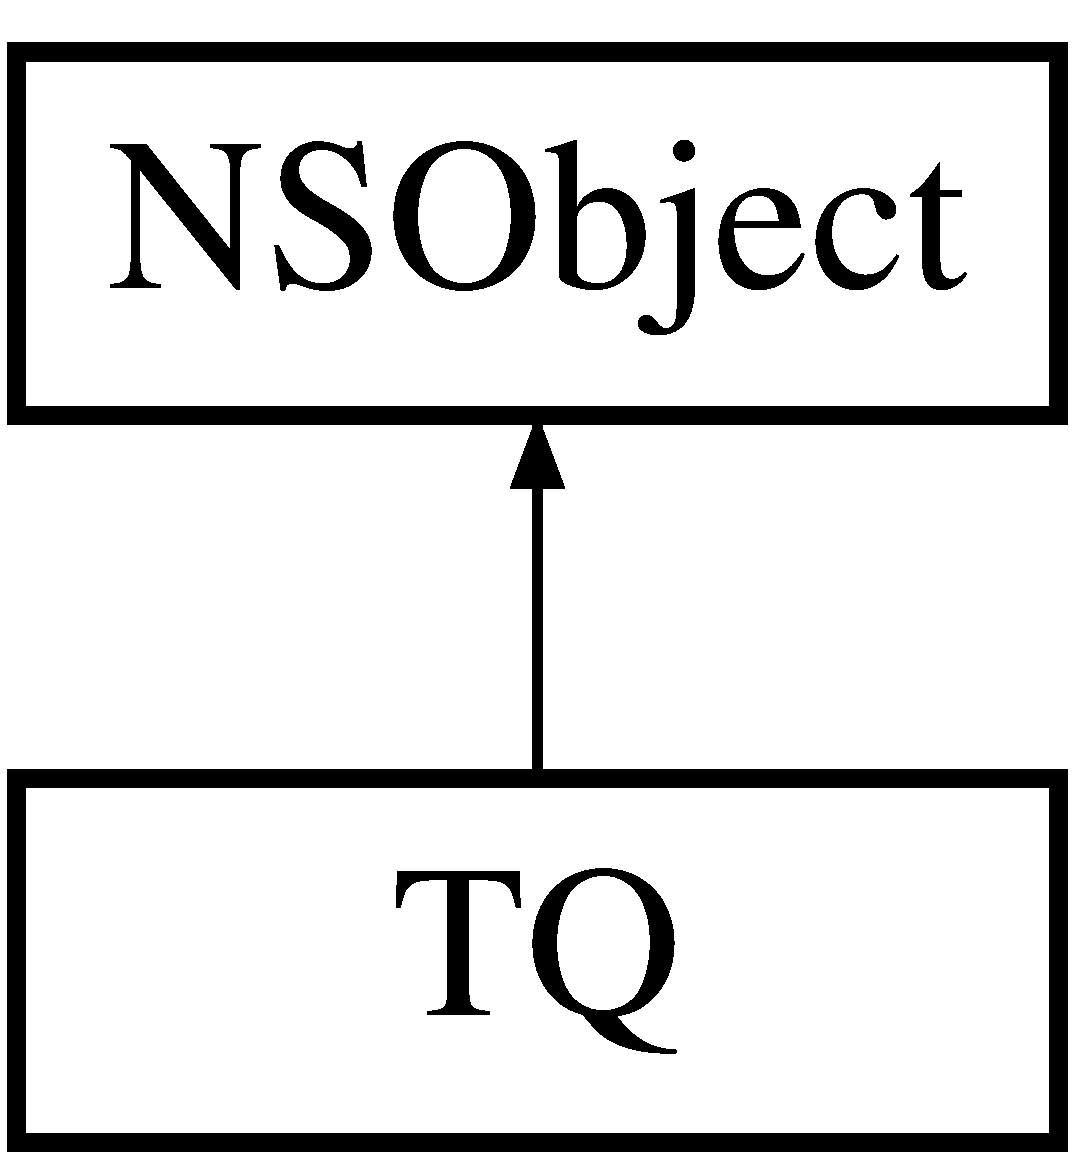
\includegraphics[height=2.000000cm]{interface_t_q}
\end{center}
\end{figure}
\subsection*{methods}
\begin{DoxyCompactItemize}
\item 
(\hyperlink{interface_t_q}{T\+Q} $\ast$) + \hyperlink{interface_t_q_a1eb13d05ac49bd6f39b5911b5290d147}{shared}
\item 
(N\+S\+String $\ast$) + \hyperlink{interface_t_q_a7d961d9f8f099fe554e99ef031b343b2}{app\+Key}
\item 
(N\+S\+String $\ast$) + \hyperlink{interface_t_q_ada9fbe4802e78b64975d51b746372665}{app\+Host}
\item 
(N\+S\+String $\ast$) + \hyperlink{interface_t_q_a1406ee198a5c9dcb87185b1b20e05269}{udid}
\item 
(N\+S\+String $\ast$) + \hyperlink{interface_t_q_a0a7336302a6134c1cdd67bc47e77a99f}{api\+Version}
\item 
(void) -\/ \hyperlink{interface_t_q_aff2f7801e1031105398e0deeae120ff3}{register\+For\+Remote\+Notification\+Types\+:delegate\+:}
\item 
(void) -\/ \hyperlink{interface_t_q_acbc578f00021d086d13947bf8f47723c}{set\+Push\+Content\+Dowload\+Automatic\+:}
\item 
(void) -\/ \hyperlink{interface_t_q_abf6c567f6548e43a77fea42da2da908b}{track\+Remote\+Nofitications\+:}
\item 
(void) -\/ \hyperlink{interface_t_q_a8cf7c68571dec41bfea63b3052745abf}{start\+With\+Key\+:and\+Environment\+:}
\item 
\hypertarget{interface_t_q_ab70ac313e849539d3f7a726618f7ee55}{}(void) -\/ {\bfseries stop}\label{interface_t_q_ab70ac313e849539d3f7a726618f7ee55}

\end{DoxyCompactItemize}


\subsection{Detailed Description}
\hyperlink{interface_t_q}{T\+Q} Holds information about the device and the app. Also, handle the initial configuration. 

\subsection{Method Documentation}
\hypertarget{interface_t_q_a0a7336302a6134c1cdd67bc47e77a99f}{}\index{T\+Q@{T\+Q}!api\+Version@{api\+Version}}
\index{api\+Version@{api\+Version}!T\+Q@{T\+Q}}
\subsubsection[{api\+Version()}]{\setlength{\rightskip}{0pt plus 5cm}+ (N\+S\+String $\ast$) api\+Version 
\begin{DoxyParamCaption}
{}
\end{DoxyParamCaption}
}\label{interface_t_q_a0a7336302a6134c1cdd67bc47e77a99f}
api\+Version

Returns the server\textquotesingle{}s A\+P\+I version.

\begin{DoxyReturn}{Returns}
the server api version. 
\end{DoxyReturn}
\hypertarget{interface_t_q_ada9fbe4802e78b64975d51b746372665}{}\index{T\+Q@{T\+Q}!app\+Host@{app\+Host}}
\index{app\+Host@{app\+Host}!T\+Q@{T\+Q}}
\subsubsection[{app\+Host()}]{\setlength{\rightskip}{0pt plus 5cm}+ (N\+S\+String $\ast$) app\+Host 
\begin{DoxyParamCaption}
{}
\end{DoxyParamCaption}
}\label{interface_t_q_ada9fbe4802e78b64975d51b746372665}
app\+Host

Returns the host of the application the app is related to.

\begin{DoxyReturn}{Returns}
host name in a string format 
\end{DoxyReturn}
\hypertarget{interface_t_q_a7d961d9f8f099fe554e99ef031b343b2}{}\index{T\+Q@{T\+Q}!app\+Key@{app\+Key}}
\index{app\+Key@{app\+Key}!T\+Q@{T\+Q}}
\subsubsection[{app\+Key()}]{\setlength{\rightskip}{0pt plus 5cm}+ (N\+S\+String $\ast$) app\+Key 
\begin{DoxyParamCaption}
{}
\end{DoxyParamCaption}
}\label{interface_t_q_a7d961d9f8f099fe554e99ef031b343b2}
app\+Key

Returns the app\+Key of the application the app is related to.

\begin{DoxyReturn}{Returns}
an string representing the app\+Key 
\end{DoxyReturn}
\hypertarget{interface_t_q_aff2f7801e1031105398e0deeae120ff3}{}\index{T\+Q@{T\+Q}!register\+For\+Remote\+Notification\+Types\+:delegate\+:@{register\+For\+Remote\+Notification\+Types\+:delegate\+:}}
\index{register\+For\+Remote\+Notification\+Types\+:delegate\+:@{register\+For\+Remote\+Notification\+Types\+:delegate\+:}!T\+Q@{T\+Q}}
\subsubsection[{register\+For\+Remote\+Notification\+Types\+:delegate\+:(int types,[delegate] id$<$ T\+Q\+Delegate $>$ delegate)}]{\setlength{\rightskip}{0pt plus 5cm}-\/ (void) register\+For\+Remote\+Notification\+Types\+: 
\begin{DoxyParamCaption}
\item[{(int)}]{types}
\item[{delegate:(id$<${\bf T\+Q\+Delegate}$>$)}]{delegate}
\end{DoxyParamCaption}
}\label{interface_t_q_aff2f7801e1031105398e0deeae120ff3}
register\+For\+Remote\+Notification\+Types delegate

Register the device to push notifications of the specified type


\begin{DoxyParams}{Parameters}
{\em types} & constant indicating the push type \\
\hline
\end{DoxyParams}
\begin{DoxySeeAlso}{See also}
\href{https://developer.apple.com/library/ios/documentation/uikit/reference/UIApplication_Class/index.html#//apple_ref/c/tdef/UIRemoteNotificationType}{\tt https\+://developer.\+apple.\+com/library/ios/documentation/uikit/reference/\+U\+I\+Application\+\_\+\+Class/index.\+html\#//apple\+\_\+ref/c/tdef/\+U\+I\+Remote\+Notification\+Type} 
\end{DoxySeeAlso}

\begin{DoxyParams}{Parameters}
{\em delegate} & any object that implements the \hyperlink{protocol_t_q_delegate-p}{T\+Q\+Delegate} protocol.\\
\hline
\end{DoxyParams}
\begin{DoxyWarning}{Warning}
this method sends \char`\"{}track\+Remote\+Notifications\char`\"{} to \hyperlink{interface_t_q}{T\+Q}. See track\+Remote\+Notifications\textquotesingle{} warnings for more information 
\end{DoxyWarning}
\hypertarget{interface_t_q_acbc578f00021d086d13947bf8f47723c}{}\index{T\+Q@{T\+Q}!set\+Push\+Content\+Dowload\+Automatic\+:@{set\+Push\+Content\+Dowload\+Automatic\+:}}
\index{set\+Push\+Content\+Dowload\+Automatic\+:@{set\+Push\+Content\+Dowload\+Automatic\+:}!T\+Q@{T\+Q}}
\subsubsection[{set\+Push\+Content\+Dowload\+Automatic\+:(\+B\+O\+O\+L automatic)}]{\setlength{\rightskip}{0pt plus 5cm}-\/ (void) set\+Push\+Content\+Dowload\+Automatic\+: 
\begin{DoxyParamCaption}
\item[{(B\+O\+O\+L)}]{automatic}
\end{DoxyParamCaption}
}\label{interface_t_q_acbc578f00021d086d13947bf8f47723c}

\begin{DoxyParams}{Parameters}
{\em automatic} & when this flag is set to true, as soon as a remote notification arrives (considering app running in background), the content is downloaded and stored in local database. When false, the application is responsible for downloading this content when the user clicks on the message. \\
\hline
\end{DoxyParams}
\hypertarget{interface_t_q_a1eb13d05ac49bd6f39b5911b5290d147}{}\index{T\+Q@{T\+Q}!shared@{shared}}
\index{shared@{shared}!T\+Q@{T\+Q}}
\subsubsection[{shared()}]{\setlength{\rightskip}{0pt plus 5cm}+ ({\bf T\+Q} $\ast$) shared 
\begin{DoxyParamCaption}
{}
\end{DoxyParamCaption}
}\label{interface_t_q_a1eb13d05ac49bd6f39b5911b5290d147}
shared Return an instance of itself, initializating it if there is no \hyperlink{interface_t_q}{T\+Q} object. Since it\textquotesingle{}s an shared object, it\textquotesingle{}ll only create one.

\begin{DoxyReturn}{Returns}
a \hyperlink{interface_t_q}{T\+Q} object 
\end{DoxyReturn}
\hypertarget{interface_t_q_a8cf7c68571dec41bfea63b3052745abf}{}\index{T\+Q@{T\+Q}!start\+With\+Key\+:and\+Environment\+:@{start\+With\+Key\+:and\+Environment\+:}}
\index{start\+With\+Key\+:and\+Environment\+:@{start\+With\+Key\+:and\+Environment\+:}!T\+Q@{T\+Q}}
\subsubsection[{start\+With\+Key\+:and\+Environment\+:(\+N\+S\+String $\ast$key,[and\+Environment] T\+Q\+Environment environment)}]{\setlength{\rightskip}{0pt plus 5cm}-\/ (void) start\+With\+Key\+: 
\begin{DoxyParamCaption}
\item[{(N\+S\+String $\ast$)}]{key}
\item[{andEnvironment:(T\+Q\+Environment)}]{environment}
\end{DoxyParamCaption}
}\label{interface_t_q_a8cf7c68571dec41bfea63b3052745abf}
start with\+Host and\+U\+D\+I\+D

Initial configuration for receiving push notifications.


\begin{DoxyParams}{Parameters}
{\em app\+Key} & the application\textquotesingle{}s appkey in string format \\
\hline
{\em udid} & the device\textquotesingle{}s udid in string format \\
\hline
{\em app\+Host} & the application\textquotesingle{}s host in string format \\
\hline
{\em api\+Version} & the server\textquotesingle{}s api version in string format\\
\hline
\end{DoxyParams}
\begin{DoxyWarning}{Warning}
Not triggered if it is not in foreground 
\end{DoxyWarning}
\hypertarget{interface_t_q_abf6c567f6548e43a77fea42da2da908b}{}\index{T\+Q@{T\+Q}!track\+Remote\+Nofitications\+:@{track\+Remote\+Nofitications\+:}}
\index{track\+Remote\+Nofitications\+:@{track\+Remote\+Nofitications\+:}!T\+Q@{T\+Q}}
\subsubsection[{track\+Remote\+Nofitications\+:(id$<$ T\+Q\+Delegate $>$ delegate)}]{\setlength{\rightskip}{0pt plus 5cm}-\/ (void) track\+Remote\+Nofitications\+: 
\begin{DoxyParamCaption}
\item[{(id$<${\bf T\+Q\+Delegate}$>$)}]{delegate}
\end{DoxyParamCaption}
}\label{interface_t_q_abf6c567f6548e43a77fea42da2da908b}
track\+Remote\+Nofitications


\begin{DoxyParams}{Parameters}
{\em delegate} & any object that implements the \hyperlink{protocol_t_q_delegate-p}{T\+Q\+Delegate} protocol.\\
\hline
\end{DoxyParams}
\begin{DoxyWarning}{Warning}
sending this message to \hyperlink{interface_t_q}{T\+Q} will substitute the given param with something else, and it\textquotesingle{}s important to call this method before sending any messages to the given delegate so the app works. 
\end{DoxyWarning}
\hypertarget{interface_t_q_a1406ee198a5c9dcb87185b1b20e05269}{}\index{T\+Q@{T\+Q}!udid@{udid}}
\index{udid@{udid}!T\+Q@{T\+Q}}
\subsubsection[{udid()}]{\setlength{\rightskip}{0pt plus 5cm}+ (N\+S\+String $\ast$) udid 
\begin{DoxyParamCaption}
{}
\end{DoxyParamCaption}
}\label{interface_t_q_a1406ee198a5c9dcb87185b1b20e05269}
udid

Returns the \textquotesingle{}unique device id\textquotesingle{} of the device.

\begin{DoxyReturn}{Returns}
the device udid. 
\end{DoxyReturn}


The documentation for this class was generated from the following files\+:\begin{DoxyCompactItemize}
\item 
T\+Q.\+h\item 
T\+Q.\+m\end{DoxyCompactItemize}

\hypertarget{category_t_q_07_08}{}\section{T\+Q() Category Reference}
\label{category_t_q_07_08}\index{T\+Q()@{T\+Q()}}
\subsection*{Protected Attributes}
\begin{DoxyCompactItemize}
\item 
\hypertarget{category_t_q_07_08_af08a5ef76671d2500b31b37636c9803c}{}T\+Q\+App\+Delegate\+Proxy $\ast$ {\bfseries \+\_\+proxy\+Delegate}\label{category_t_q_07_08_af08a5ef76671d2500b31b37636c9803c}

\item 
\hypertarget{category_t_q_07_08_aa089f3f44f503078b0f07322641e9779}{}double {\bfseries unsent\+Session\+Length}\label{category_t_q_07_08_aa089f3f44f503078b0f07322641e9779}

\item 
\hypertarget{category_t_q_07_08_a8b3692c0912666dc015bacaa47c4119f}{}N\+S\+Timer $\ast$ {\bfseries timer}\label{category_t_q_07_08_a8b3692c0912666dc015bacaa47c4119f}

\item 
\hypertarget{category_t_q_07_08_a56ae20b439c4254040761c1364005eba}{}double {\bfseries last\+Time}\label{category_t_q_07_08_a56ae20b439c4254040761c1364005eba}

\item 
\hypertarget{category_t_q_07_08_a1805b83b9be1d506fc0b280feb885742}{}B\+O\+O\+L {\bfseries is\+Suspended}\label{category_t_q_07_08_a1805b83b9be1d506fc0b280feb885742}

\end{DoxyCompactItemize}


The documentation for this category was generated from the following file\+:\begin{DoxyCompactItemize}
\item 
T\+Q.\+m\end{DoxyCompactItemize}

\hypertarget{interface_t_q_analytics}{}\section{T\+Q\+Analytics Class Reference}
\label{interface_t_q_analytics}\index{T\+Q\+Analytics@{T\+Q\+Analytics}}


{\ttfamily \#import $<$T\+Q\+Analytics.\+h$>$}

Inheritance diagram for T\+Q\+Analytics\+:\begin{figure}[H]
\begin{center}
\leavevmode
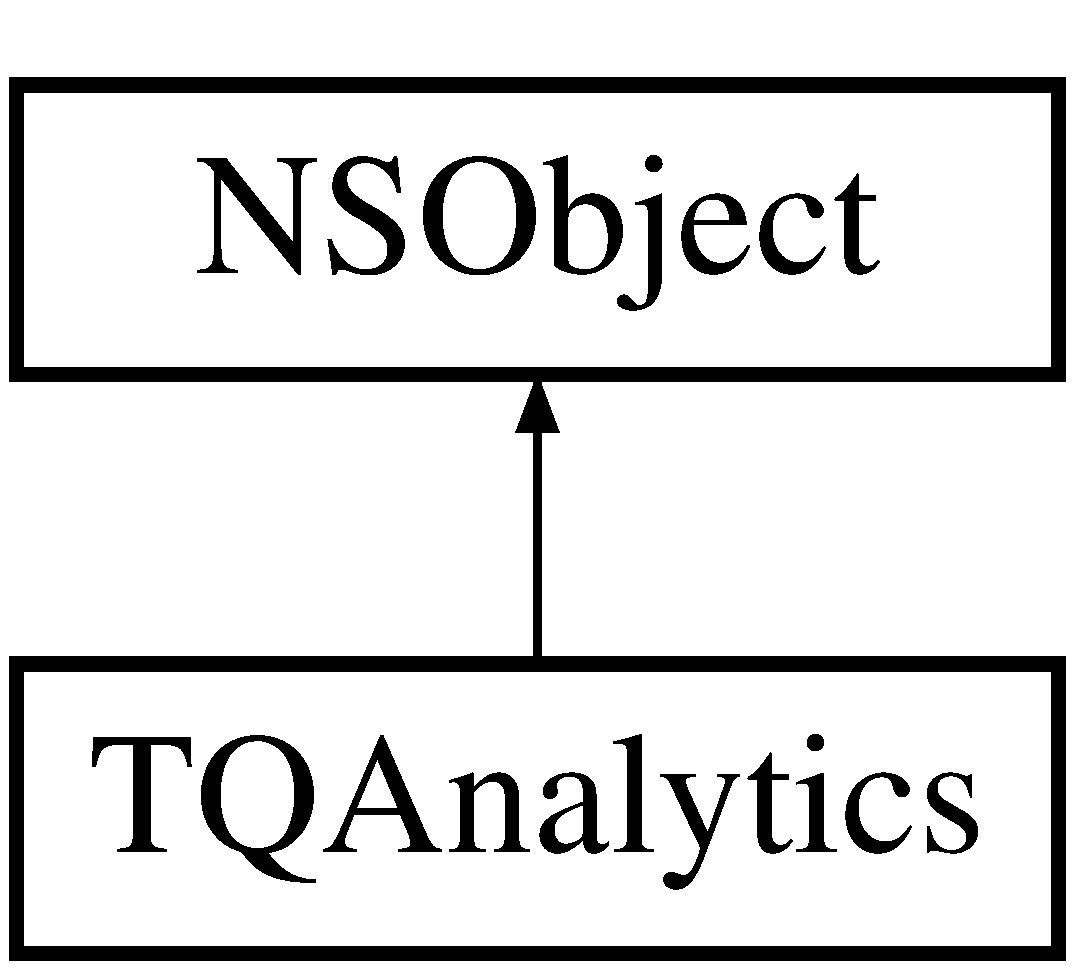
\includegraphics[height=2.000000cm]{interface_t_q_analytics}
\end{center}
\end{figure}
\subsection*{Instance Methods}
\begin{DoxyCompactItemize}
\item 
(void) -\/ \hyperlink{interface_t_q_analytics_a91c06faeb927363c040b516ed195449c}{record\+Social}
\item 
(void) -\/ \hyperlink{interface_t_q_analytics_a27858a475fc0338c9975e32b0bb21f12}{add\+Bluetooh\+State\+To\+Connection\+Queue\+:}
\end{DoxyCompactItemize}
\begin{Indent}{\bf event recording}\par
\begin{DoxyCompactItemize}
\item 
(void) -\/ \hyperlink{interface_t_q_analytics_ae399bfa3974b8464f6bf475657e62363}{record\+Event\+:count\+:}
\item 
(void) -\/ \hyperlink{interface_t_q_analytics_a904f5ef03adb907dd15c0a1c6805caaf}{record\+Event\+:segmentation\+:count\+:}
\end{DoxyCompactItemize}
\end{Indent}
\begin{Indent}{\bf Custom data}\par
\begin{DoxyCompactItemize}
\item 
(void) -\/ \hyperlink{interface_t_q_analytics_aa5ca45a7be910512ad72cbfe70a005e3}{add\+Custom\+Data\+:completion\+:}
\item 
(void) -\/ \hyperlink{interface_t_q_analytics_a5a882188abdb0b24adcbaa1e2c6ecec0}{add\+Custom\+Data\+:keys\+To\+Ignore\+:completion\+:}
\item 
(void) -\/ \hyperlink{interface_t_q_analytics_a98186f450231638021ad14fc771163f6}{update\+Settings}
\end{DoxyCompactItemize}
\end{Indent}
\begin{Indent}{\bf Custom status}\par
\begin{DoxyCompactItemize}
\item 
(void) -\/ \hyperlink{interface_t_q_analytics_a04fa7504b4a51fd75b8fc52494009179}{update\+Status\+:status\+:completion\+:}
\end{DoxyCompactItemize}
\end{Indent}
\begin{Indent}{\bf Custom action}\par
\begin{DoxyCompactItemize}
\item 
(void) -\/ \hyperlink{interface_t_q_analytics_ab6b929f63a2224dc0b33d5d7ad2c9b58}{send\+Action\+Choosen\+:pid\+:completion\+:}
\end{DoxyCompactItemize}
\end{Indent}
\begin{Indent}{\bf Timer handles}\par
\begin{DoxyCompactItemize}
\item 
(void) -\/ \hyperlink{interface_t_q_analytics_adfaf41d8f2679048b42a5d8ef33c465e}{start}
\item 
(void) -\/ \hyperlink{interface_t_q_analytics_ab2ab8cdc4c1ae2ea016377475edd7b6e}{suspend}
\item 
(void) -\/ \hyperlink{interface_t_q_analytics_aa8acff938c3f1a83a44232e3a3937879}{resume}
\item 
(void) -\/ \hyperlink{interface_t_q_analytics_add562e365bbe96e0e09cf59e26fbe883}{exit}
\end{DoxyCompactItemize}
\end{Indent}
\subsection*{Class Methods}
\begin{DoxyCompactItemize}
\item 
(\hyperlink{interface_t_q_analytics}{T\+Q\+Analytics} $\ast$) + \hyperlink{interface_t_q_analytics_a2a196611c33fe847e9e0cd06748a508d}{shared}
\end{DoxyCompactItemize}


\subsection{Detailed Description}
\hyperlink{interface_t_q_analytics}{T\+Q\+Analytics} Handle analytical data and it\textquotesingle{}s retrieval through periodic actions. 

\subsection{Method Documentation}
\hypertarget{interface_t_q_analytics_a27858a475fc0338c9975e32b0bb21f12}{}\index{T\+Q\+Analytics@{T\+Q\+Analytics}!add\+Bluetooh\+State\+To\+Connection\+Queue\+:@{add\+Bluetooh\+State\+To\+Connection\+Queue\+:}}
\index{add\+Bluetooh\+State\+To\+Connection\+Queue\+:@{add\+Bluetooh\+State\+To\+Connection\+Queue\+:}!T\+Q\+Analytics@{T\+Q\+Analytics}}
\subsubsection[{add\+Bluetooh\+State\+To\+Connection\+Queue\+:(\+B\+O\+O\+L state)}]{\setlength{\rightskip}{0pt plus 5cm}-\/ (void) add\+Bluetooh\+State\+To\+Connection\+Queue\+: 
\begin{DoxyParamCaption}
\item[{(B\+O\+O\+L)}]{state}
\end{DoxyParamCaption}
}\label{interface_t_q_analytics_a27858a475fc0338c9975e32b0bb21f12}
add\+Bluetooh\+State\+To\+Connection\+Queue \hypertarget{interface_t_q_analytics_aa5ca45a7be910512ad72cbfe70a005e3}{}\index{T\+Q\+Analytics@{T\+Q\+Analytics}!add\+Custom\+Data\+:completion\+:@{add\+Custom\+Data\+:completion\+:}}
\index{add\+Custom\+Data\+:completion\+:@{add\+Custom\+Data\+:completion\+:}!T\+Q\+Analytics@{T\+Q\+Analytics}}
\subsubsection[{add\+Custom\+Data\+:completion\+:(\+N\+S\+Dictionary $\ast$custom\+Data,[completion] void($^\wedge$completion)(\+B\+O\+O\+L success))}]{\setlength{\rightskip}{0pt plus 5cm}-\/ (void) add\+Custom\+Data\+: 
\begin{DoxyParamCaption}
\item[{(N\+S\+Dictionary $\ast$)}]{custom\+Data}
\item[{completion:(void($^\wedge$)(B\+O\+O\+L success))}]{completion}
\end{DoxyParamCaption}
}\label{interface_t_q_analytics_aa5ca45a7be910512ad72cbfe70a005e3}
add\+Custom\+Data custom\+Data completion Add device\textquotesingle{}s custom data at our A\+P\+I. Note that it\textquotesingle{}ll override any existing data already added.


\begin{DoxyParams}{Parameters}
{\em custom\+Data} & A N\+S\+Dictionary containing a J\+S\+O\+N representation of custom data to be added. Keys must be string and values can only be Strings, Integers or Doubles \\
\hline
{\em completion} & A block that is executed when the upload request has completed. The success block parameter indicates whether the data was uploaded or not. \\
\hline
\end{DoxyParams}
\hypertarget{interface_t_q_analytics_a5a882188abdb0b24adcbaa1e2c6ecec0}{}\index{T\+Q\+Analytics@{T\+Q\+Analytics}!add\+Custom\+Data\+:keys\+To\+Ignore\+:completion\+:@{add\+Custom\+Data\+:keys\+To\+Ignore\+:completion\+:}}
\index{add\+Custom\+Data\+:keys\+To\+Ignore\+:completion\+:@{add\+Custom\+Data\+:keys\+To\+Ignore\+:completion\+:}!T\+Q\+Analytics@{T\+Q\+Analytics}}
\subsubsection[{add\+Custom\+Data\+:keys\+To\+Ignore\+:completion\+:(\+N\+S\+Dictionary $\ast$custom\+Data,[keys\+To\+Ignore] N\+S\+Array $\ast$keys\+To\+Ignore,[completion] void($^\wedge$completion)(\+B\+O\+O\+L success))}]{\setlength{\rightskip}{0pt plus 5cm}-\/ (void) add\+Custom\+Data\+: 
\begin{DoxyParamCaption}
\item[{(N\+S\+Dictionary $\ast$)}]{custom\+Data}
\item[{keysToIgnore:(N\+S\+Array $\ast$)}]{keys\+To\+Ignore}
\item[{completion:(void($^\wedge$)(B\+O\+O\+L success))}]{completion}
\end{DoxyParamCaption}
}\label{interface_t_q_analytics_a5a882188abdb0b24adcbaa1e2c6ecec0}
add\+Custom\+Data custom\+Data completion Add device\textquotesingle{}s custom data at our A\+P\+I. Note that it\textquotesingle{}ll override any existing data already added.


\begin{DoxyParams}{Parameters}
{\em custom\+Data} & A N\+S\+Dictionary containing a J\+S\+O\+N representation of custom data to be added. Keys must be string and values can only be Strings, Integers or Doubles \\
\hline
{\em keys\+To\+Ignore} & An array of strings with the keys that should be ignored when adding the data filters. Data that is too sparse M\+U\+S\+T be ignored, like User Ids for example \\
\hline
{\em completion} & A block that is executed when the upload request has completed. The success block parameter indicates whether the data was uploaded or not. \\
\hline
\end{DoxyParams}
\hypertarget{interface_t_q_analytics_add562e365bbe96e0e09cf59e26fbe883}{}\index{T\+Q\+Analytics@{T\+Q\+Analytics}!exit@{exit}}
\index{exit@{exit}!T\+Q\+Analytics@{T\+Q\+Analytics}}
\subsubsection[{exit()}]{\setlength{\rightskip}{0pt plus 5cm}-\/ (void) exit 
\begin{DoxyParamCaption}
{}
\end{DoxyParamCaption}
}\label{interface_t_q_analytics_add562e365bbe96e0e09cf59e26fbe883}
exit does nothing. \hypertarget{interface_t_q_analytics_ae399bfa3974b8464f6bf475657e62363}{}\index{T\+Q\+Analytics@{T\+Q\+Analytics}!record\+Event\+:count\+:@{record\+Event\+:count\+:}}
\index{record\+Event\+:count\+:@{record\+Event\+:count\+:}!T\+Q\+Analytics@{T\+Q\+Analytics}}
\subsubsection[{record\+Event\+:count\+:(\+N\+S\+String $\ast$event,[count] int count)}]{\setlength{\rightskip}{0pt plus 5cm}-\/ (void) record\+Event\+: 
\begin{DoxyParamCaption}
\item[{(N\+S\+String $\ast$)}]{event}
\item[{count:(int)}]{count}
\end{DoxyParamCaption}
}\label{interface_t_q_analytics_ae399bfa3974b8464f6bf475657e62363}
record\+Event count Record an event\textquotesingle{}s count, adding it to the previous count.


\begin{DoxyParams}{Parameters}
{\em event} & The event\textquotesingle{}s name \\
\hline
{\em count} & the count to be added \\
\hline
\end{DoxyParams}
\hypertarget{interface_t_q_analytics_a904f5ef03adb907dd15c0a1c6805caaf}{}\index{T\+Q\+Analytics@{T\+Q\+Analytics}!record\+Event\+:segmentation\+:count\+:@{record\+Event\+:segmentation\+:count\+:}}
\index{record\+Event\+:segmentation\+:count\+:@{record\+Event\+:segmentation\+:count\+:}!T\+Q\+Analytics@{T\+Q\+Analytics}}
\subsubsection[{record\+Event\+:segmentation\+:count\+:(\+N\+S\+String $\ast$event,[segmentation] N\+S\+Dictionary $\ast$segmentation,[count] int count)}]{\setlength{\rightskip}{0pt plus 5cm}-\/ (void) record\+Event\+: 
\begin{DoxyParamCaption}
\item[{(N\+S\+String $\ast$)}]{event}
\item[{segmentation:(N\+S\+Dictionary $\ast$)}]{segmentation}
\item[{count:(int)}]{count}
\end{DoxyParamCaption}
}\label{interface_t_q_analytics_a904f5ef03adb907dd15c0a1c6805caaf}
record\+Event segmentation count Record an event\textquotesingle{}s count, adding it to the previous count.


\begin{DoxyParams}{Parameters}
{\em event} & The event\textquotesingle{}s name \\
\hline
{\em count} & the count to be added \\
\hline
{\em segmentation} & adicional information about the event \\
\hline
\end{DoxyParams}
\hypertarget{interface_t_q_analytics_a91c06faeb927363c040b516ed195449c}{}\index{T\+Q\+Analytics@{T\+Q\+Analytics}!record\+Social@{record\+Social}}
\index{record\+Social@{record\+Social}!T\+Q\+Analytics@{T\+Q\+Analytics}}
\subsubsection[{record\+Social()}]{\setlength{\rightskip}{0pt plus 5cm}-\/ (void) record\+Social 
\begin{DoxyParamCaption}
{}
\end{DoxyParamCaption}
}\label{interface_t_q_analytics_a91c06faeb927363c040b516ed195449c}
record\+Social Records the social data (facebook) if an facebook session is initiated. It records the facebook\+Id, gender and age of the user. \hypertarget{interface_t_q_analytics_aa8acff938c3f1a83a44232e3a3937879}{}\index{T\+Q\+Analytics@{T\+Q\+Analytics}!resume@{resume}}
\index{resume@{resume}!T\+Q\+Analytics@{T\+Q\+Analytics}}
\subsubsection[{resume()}]{\setlength{\rightskip}{0pt plus 5cm}-\/ (void) resume 
\begin{DoxyParamCaption}
{}
\end{DoxyParamCaption}
}\label{interface_t_q_analytics_aa8acff938c3f1a83a44232e3a3937879}
suspend resume the timer. \hypertarget{interface_t_q_analytics_ab6b929f63a2224dc0b33d5d7ad2c9b58}{}\index{T\+Q\+Analytics@{T\+Q\+Analytics}!send\+Action\+Choosen\+:pid\+:completion\+:@{send\+Action\+Choosen\+:pid\+:completion\+:}}
\index{send\+Action\+Choosen\+:pid\+:completion\+:@{send\+Action\+Choosen\+:pid\+:completion\+:}!T\+Q\+Analytics@{T\+Q\+Analytics}}
\subsubsection[{send\+Action\+Choosen\+:pid\+:completion\+:(\+N\+S\+String $\ast$button\+Choosen,[pid] N\+S\+String $\ast$pid,[completion] void($^\wedge$completion)(\+B\+O\+O\+L success))}]{\setlength{\rightskip}{0pt plus 5cm}-\/ (void) send\+Action\+Choosen\+: 
\begin{DoxyParamCaption}
\item[{(N\+S\+String $\ast$)}]{button\+Choosen}
\item[{pid:(N\+S\+String $\ast$)}]{pid}
\item[{completion:(void($^\wedge$)(B\+O\+O\+L success))}]{completion}
\end{DoxyParamCaption}
}\label{interface_t_q_analytics_ab6b929f63a2224dc0b33d5d7ad2c9b58}
send\+Action\+Choosen button\+Choosen pid completion Add push notification\textquotesingle{}s custom status at our A\+P\+I.


\begin{DoxyParams}{Parameters}
{\em button\+Choosen} & A custom action button choosen. \\
\hline
{\em pid} & A string with the push notification id for which should be added the custom status. \\
\hline
{\em completion} & A block that is executed when the upload request has completed. The success block parameter indicates whether the status was uploaded or not. \\
\hline
\end{DoxyParams}
\hypertarget{interface_t_q_analytics_a2a196611c33fe847e9e0cd06748a508d}{}\index{T\+Q\+Analytics@{T\+Q\+Analytics}!shared@{shared}}
\index{shared@{shared}!T\+Q\+Analytics@{T\+Q\+Analytics}}
\subsubsection[{shared()}]{\setlength{\rightskip}{0pt plus 5cm}+ ({\bf T\+Q\+Analytics} $\ast$) shared 
\begin{DoxyParamCaption}
{}
\end{DoxyParamCaption}
}\label{interface_t_q_analytics_a2a196611c33fe847e9e0cd06748a508d}
shared Return an instance of itself, initializating it if there is no \hyperlink{interface_t_q_analytics}{T\+Q\+Analytics} object. Since it\textquotesingle{}s an shared object, it\textquotesingle{}ll only create one.

\begin{DoxyReturn}{Returns}
a \hyperlink{interface_t_q_analytics}{T\+Q\+Analytics} object 
\end{DoxyReturn}
\hypertarget{interface_t_q_analytics_adfaf41d8f2679048b42a5d8ef33c465e}{}\index{T\+Q\+Analytics@{T\+Q\+Analytics}!start@{start}}
\index{start@{start}!T\+Q\+Analytics@{T\+Q\+Analytics}}
\subsubsection[{start()}]{\setlength{\rightskip}{0pt plus 5cm}-\/ (void) start 
\begin{DoxyParamCaption}
{}
\end{DoxyParamCaption}
}\label{interface_t_q_analytics_adfaf41d8f2679048b42a5d8ef33c465e}
start starts the timer for periodic actions. \hypertarget{interface_t_q_analytics_ab2ab8cdc4c1ae2ea016377475edd7b6e}{}\index{T\+Q\+Analytics@{T\+Q\+Analytics}!suspend@{suspend}}
\index{suspend@{suspend}!T\+Q\+Analytics@{T\+Q\+Analytics}}
\subsubsection[{suspend()}]{\setlength{\rightskip}{0pt plus 5cm}-\/ (void) suspend 
\begin{DoxyParamCaption}
{}
\end{DoxyParamCaption}
}\label{interface_t_q_analytics_ab2ab8cdc4c1ae2ea016377475edd7b6e}
suspend suspends the timer. \hypertarget{interface_t_q_analytics_a98186f450231638021ad14fc771163f6}{}\index{T\+Q\+Analytics@{T\+Q\+Analytics}!update\+Settings@{update\+Settings}}
\index{update\+Settings@{update\+Settings}!T\+Q\+Analytics@{T\+Q\+Analytics}}
\subsubsection[{update\+Settings()}]{\setlength{\rightskip}{0pt plus 5cm}-\/ (void) update\+Settings 
\begin{DoxyParamCaption}
{}
\end{DoxyParamCaption}
}\label{interface_t_q_analytics_a98186f450231638021ad14fc771163f6}
update\+Settings Send current settings (\char`\"{}location enabled\char`\"{} and \char`\"{}push enabled\char`\"{}) to api in order to update them. \hypertarget{interface_t_q_analytics_a04fa7504b4a51fd75b8fc52494009179}{}\index{T\+Q\+Analytics@{T\+Q\+Analytics}!update\+Status\+:status\+:completion\+:@{update\+Status\+:status\+:completion\+:}}
\index{update\+Status\+:status\+:completion\+:@{update\+Status\+:status\+:completion\+:}!T\+Q\+Analytics@{T\+Q\+Analytics}}
\subsubsection[{update\+Status\+:status\+:completion\+:(\+N\+S\+String $\ast$pid,[status] N\+S\+String $\ast$status,[completion] void($^\wedge$completion)(\+B\+O\+O\+L success))}]{\setlength{\rightskip}{0pt plus 5cm}-\/ (void) update\+Status\+: 
\begin{DoxyParamCaption}
\item[{(N\+S\+String $\ast$)}]{pid}
\item[{status:(N\+S\+String $\ast$)}]{status}
\item[{completion:(void($^\wedge$)(B\+O\+O\+L success))}]{completion}
\end{DoxyParamCaption}
}\label{interface_t_q_analytics_a04fa7504b4a51fd75b8fc52494009179}
update\+Status pid status completion Add push notification\textquotesingle{}s custom status at our A\+P\+I.


\begin{DoxyParams}{Parameters}
{\em pid} & A string with the push notification id for which should be added the custom status. \\
\hline
{\em status} & A custom status name that was trigged by the push notification. \\
\hline
{\em completion} & A block that is executed when the upload request has completed. The success block parameter indicates whether the status was uploaded or not. \\
\hline
\end{DoxyParams}


The documentation for this class was generated from the following files\+:\begin{DoxyCompactItemize}
\item 
T\+Q\+Analytics.\+h\item 
T\+Q\+Analytics.\+m\end{DoxyCompactItemize}

\hypertarget{category_t_q_analytics_07_08}{}\section{T\+Q\+Analytics() Category Reference}
\label{category_t_q_analytics_07_08}\index{T\+Q\+Analytics()@{T\+Q\+Analytics()}}
\subsection*{Protected Attributes}
\begin{DoxyCompactItemize}
\item 
\hypertarget{category_t_q_analytics_07_08_acbc6c029260e9cf5d8727cc9fa4078f5}{}N\+S\+String $\ast$ {\bfseries controller}\label{category_t_q_analytics_07_08_acbc6c029260e9cf5d8727cc9fa4078f5}

\item 
\hypertarget{category_t_q_analytics_07_08_a8b0e6aeb25af63547e61f7099689ab19}{}double {\bfseries unsent\+Session\+Length}\label{category_t_q_analytics_07_08_a8b0e6aeb25af63547e61f7099689ab19}

\item 
\hypertarget{category_t_q_analytics_07_08_aa785b246cb64a8d2e15ff03505903e4c}{}N\+S\+Timer $\ast$ {\bfseries timer}\label{category_t_q_analytics_07_08_aa785b246cb64a8d2e15ff03505903e4c}

\item 
\hypertarget{category_t_q_analytics_07_08_a9f58f193913088c83d7b6e881e8b3af0}{}double {\bfseries last\+Time}\label{category_t_q_analytics_07_08_a9f58f193913088c83d7b6e881e8b3af0}

\item 
\hypertarget{category_t_q_analytics_07_08_a8c68953b32c9d61cd3ee042d23dc153e}{}B\+O\+O\+L {\bfseries is\+Suspended}\label{category_t_q_analytics_07_08_a8c68953b32c9d61cd3ee042d23dc153e}

\item 
\hypertarget{category_t_q_analytics_07_08_a041b5bc2f50e6ae878aaf1dad0c34f7d}{}T\+Q\+Event\+Queue $\ast$ {\bfseries event\+Queue}\label{category_t_q_analytics_07_08_a041b5bc2f50e6ae878aaf1dad0c34f7d}

\item 
\hypertarget{category_t_q_analytics_07_08_af7832fb2fba23062f43347ae5c731724}{}T\+Q\+Social\+Info $\ast$ {\bfseries social\+Info}\label{category_t_q_analytics_07_08_af7832fb2fba23062f43347ae5c731724}

\end{DoxyCompactItemize}


The documentation for this category was generated from the following file\+:\begin{DoxyCompactItemize}
\item 
T\+Q\+Analytics.\+m\end{DoxyCompactItemize}

\hypertarget{protocol_t_q_delegate-p}{}\section{$<$T\+Q\+Delegate$>$ Protocol Reference}
\label{protocol_t_q_delegate-p}\index{$<$\+T\+Q\+Delegate$>$@{$<$\+T\+Q\+Delegate$>$}}
Inheritance diagram for $<$T\+Q\+Delegate$>$\+:\begin{figure}[H]
\begin{center}
\leavevmode
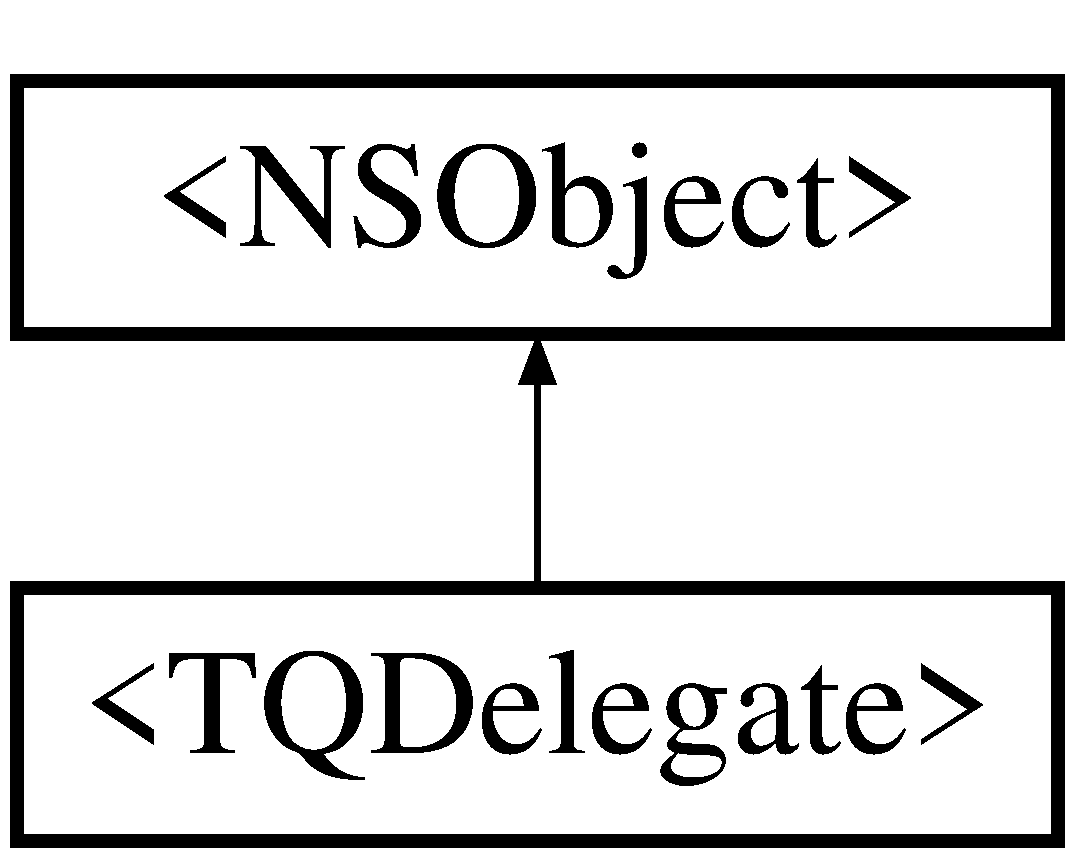
\includegraphics[height=2.000000cm]{protocol_t_q_delegate-p}
\end{center}
\end{figure}
\subsection*{Instance Methods}
\begin{DoxyCompactItemize}
\item 
\hypertarget{protocol_t_q_delegate-p_a34747cffd0d6cc29542fbcd96c92d470}{}(void) -\/ {\bfseries handle\+Foreground\+Push\+Notification\+:push\+Id\+:}\label{protocol_t_q_delegate-p_a34747cffd0d6cc29542fbcd96c92d470}

\item 
\hypertarget{protocol_t_q_delegate-p_a2d73eca46f921692a73671d3f330be15}{}(void) -\/ {\bfseries handle\+Background\+Push\+Notification\+:push\+Id\+:}\label{protocol_t_q_delegate-p_a2d73eca46f921692a73671d3f330be15}

\item 
\hypertarget{protocol_t_q_delegate-p_a10a20e42ddc351e3a62ee90e7c8830f5}{}(void) -\/ {\bfseries handle\+Custom\+Action\+With\+Identifier\+:push\+Id\+:}\label{protocol_t_q_delegate-p_a10a20e42ddc351e3a62ee90e7c8830f5}

\end{DoxyCompactItemize}


The documentation for this protocol was generated from the following file\+:\begin{DoxyCompactItemize}
\item 
T\+Q.\+h\end{DoxyCompactItemize}

\hypertarget{interface_t_q_geotrigger}{}\section{T\+Q\+Geotrigger Class Reference}
\label{interface_t_q_geotrigger}\index{T\+Q\+Geotrigger@{T\+Q\+Geotrigger}}


{\ttfamily \#import $<$T\+Q\+Geotrigger.\+h$>$}

Inheritance diagram for T\+Q\+Geotrigger\+:\begin{figure}[H]
\begin{center}
\leavevmode
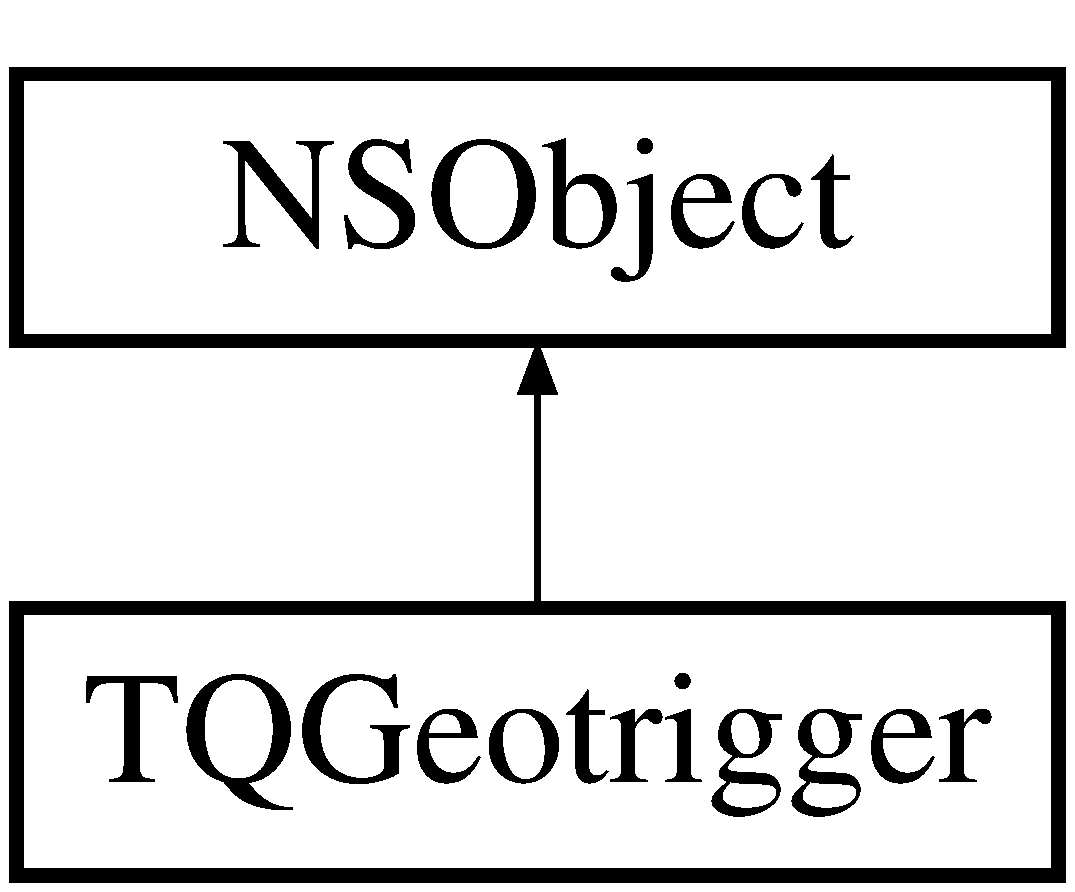
\includegraphics[height=2.000000cm]{interface_t_q_geotrigger}
\end{center}
\end{figure}
\subsection*{Instance Methods}
\begin{DoxyCompactItemize}
\item 
(void) -\/ \hyperlink{interface_t_q_geotrigger_a373e03146f521ac53815ed3fa3d6d52e}{configure\+With\+Client\+Id\+:and\+Tags\+:and\+Completion\+Handler\+:}
\item 
(void) -\/ \hyperlink{interface_t_q_geotrigger_adab731af1533f72250348dea657301ce}{start\+Geotrigger\+Service}
\item 
(void) -\/ \hyperlink{interface_t_q_geotrigger_a730fde8f6f5e22db8785bab538c8aea9}{stop\+Geotrigger\+Service}
\item 
(void) -\/ \hyperlink{interface_t_q_geotrigger_a5feb3e0d3d3a4482ad968fefca944a92}{start\+Geotrigger\+Service\+:with\+Tags\+:}
\item 
(void) -\/ \hyperlink{interface_t_q_geotrigger_a265cb2de297e4a87eb43f592e05e50d8}{stop\+Geotrigger\+Service\+:with\+Tags\+:}
\item 
(void) -\/ \hyperlink{interface_t_q_geotrigger_aebbef6b764f07609971eaf67f39cd368}{resume\+Geotrigger\+Service}
\item 
(void) -\/ \hyperlink{interface_t_q_geotrigger_ae4539d4aede1b633322bacc8432d0195}{pause\+Geotrigger\+Service}
\item 
(void) -\/ \hyperlink{interface_t_q_geotrigger_abf215acd1e6afcbae1d768452b15d1d3}{request\+Geofences\+:completion\+:}
\end{DoxyCompactItemize}
\subsection*{Class Methods}
\begin{DoxyCompactItemize}
\item 
(\hyperlink{interface_t_q_geotrigger}{T\+Q\+Geotrigger} $\ast$) + \hyperlink{interface_t_q_geotrigger_a73a5441f01b4622a652f9f9fabb04039}{shared}
\item 
(N\+S\+String $\ast$) + \hyperlink{interface_t_q_geotrigger_ab02b5f4479c7519958ab401c637adc93}{tracking\+Id}
\end{DoxyCompactItemize}


\subsection{Detailed Description}
\hyperlink{interface_t_q_geotrigger}{T\+Q\+Geotrigger} Simply commands when to start and when to stop the geotrigger service 

\subsection{Method Documentation}
\hypertarget{interface_t_q_geotrigger_a373e03146f521ac53815ed3fa3d6d52e}{}\index{T\+Q\+Geotrigger@{T\+Q\+Geotrigger}!configure\+With\+Client\+Id\+:and\+Tags\+:and\+Completion\+Handler\+:@{configure\+With\+Client\+Id\+:and\+Tags\+:and\+Completion\+Handler\+:}}
\index{configure\+With\+Client\+Id\+:and\+Tags\+:and\+Completion\+Handler\+:@{configure\+With\+Client\+Id\+:and\+Tags\+:and\+Completion\+Handler\+:}!T\+Q\+Geotrigger@{T\+Q\+Geotrigger}}
\subsubsection[{configure\+With\+Client\+Id\+:and\+Tags\+:and\+Completion\+Handler\+:(\+N\+S\+String $\ast$client\+Id,[and\+Tags] N\+S\+Array $\ast$tags,[and\+Completion\+Handler] void($^\wedge$completion\+Handler)(void))}]{\setlength{\rightskip}{0pt plus 5cm}-\/ (void) configure\+With\+Client\+Id\+: 
\begin{DoxyParamCaption}
\item[{(N\+S\+String $\ast$)}]{client\+Id}
\item[{andTags:(N\+S\+Array $\ast$)}]{tags}
\item[{andCompletionHandler:(void($^\wedge$)(void))}]{completion\+Handler}
\end{DoxyParamCaption}
}\label{interface_t_q_geotrigger_a373e03146f521ac53815ed3fa3d6d52e}
configure\+With\+Client\+Id and Tags Initialize Geotrigger constants


\begin{DoxyParams}{Parameters}
{\em client\+Id} & the client Id \\
\hline
{\em tags} & An optional list of tags to be set on the device after it registers itself \\
\hline
\end{DoxyParams}
\begin{DoxySeeAlso}{See also}
\href{https://developers.arcgis.com/geotrigger-service/ios-reference/Classes/AGSGTGeotriggerManager.html#//api/name/setupWithClientId:trackingProfile:registerForRemoteNotifications:isProduction:tags:completion:}{\tt https\+://developers.\+arcgis.\+com/geotrigger-\/service/ios-\/reference/\+Classes/\+A\+G\+S\+G\+T\+Geotrigger\+Manager.\+html\#//api/name/setup\+With\+Client\+Id\+:tracking\+Profile\+:register\+For\+Remote\+Notifications\+:is\+Production\+:tags\+:completion\+:} 
\end{DoxySeeAlso}
\hypertarget{interface_t_q_geotrigger_ae4539d4aede1b633322bacc8432d0195}{}\index{T\+Q\+Geotrigger@{T\+Q\+Geotrigger}!pause\+Geotrigger\+Service@{pause\+Geotrigger\+Service}}
\index{pause\+Geotrigger\+Service@{pause\+Geotrigger\+Service}!T\+Q\+Geotrigger@{T\+Q\+Geotrigger}}
\subsubsection[{pause\+Geotrigger\+Service()}]{\setlength{\rightskip}{0pt plus 5cm}-\/ (void) pause\+Geotrigger\+Service 
\begin{DoxyParamCaption}
{}
\end{DoxyParamCaption}
}\label{interface_t_q_geotrigger_ae4539d4aede1b633322bacc8432d0195}
pause\+Geotrigger\+Service Stops the geotrigger service on i\+O\+S 8+ for the cases when location usage is only authorized when app is being used \hypertarget{interface_t_q_geotrigger_abf215acd1e6afcbae1d768452b15d1d3}{}\index{T\+Q\+Geotrigger@{T\+Q\+Geotrigger}!request\+Geofences\+:completion\+:@{request\+Geofences\+:completion\+:}}
\index{request\+Geofences\+:completion\+:@{request\+Geofences\+:completion\+:}!T\+Q\+Geotrigger@{T\+Q\+Geotrigger}}
\subsubsection[{request\+Geofences\+:completion\+:(int page,[completion] void($^\wedge$completion)(\+N\+S\+Array $\ast$data))}]{\setlength{\rightskip}{0pt plus 5cm}-\/ (void) request\+Geofences\+: 
\begin{DoxyParamCaption}
\item[{(int)}]{page}
\item[{completion:(void($^\wedge$)(N\+S\+Array $\ast$data))}]{completion}
\end{DoxyParamCaption}
}\label{interface_t_q_geotrigger_abf215acd1e6afcbae1d768452b15d1d3}
request\+Geofences gets all app Geofences

\begin{DoxyReturn}{Returns}
an Geofences array 
\end{DoxyReturn}
\hypertarget{interface_t_q_geotrigger_aebbef6b764f07609971eaf67f39cd368}{}\index{T\+Q\+Geotrigger@{T\+Q\+Geotrigger}!resume\+Geotrigger\+Service@{resume\+Geotrigger\+Service}}
\index{resume\+Geotrigger\+Service@{resume\+Geotrigger\+Service}!T\+Q\+Geotrigger@{T\+Q\+Geotrigger}}
\subsubsection[{resume\+Geotrigger\+Service()}]{\setlength{\rightskip}{0pt plus 5cm}-\/ (void) resume\+Geotrigger\+Service 
\begin{DoxyParamCaption}
{}
\end{DoxyParamCaption}
}\label{interface_t_q_geotrigger_aebbef6b764f07609971eaf67f39cd368}
resume\+Geotrigger\+Service Starts the geotrigger service \hypertarget{interface_t_q_geotrigger_a73a5441f01b4622a652f9f9fabb04039}{}\index{T\+Q\+Geotrigger@{T\+Q\+Geotrigger}!shared@{shared}}
\index{shared@{shared}!T\+Q\+Geotrigger@{T\+Q\+Geotrigger}}
\subsubsection[{shared()}]{\setlength{\rightskip}{0pt plus 5cm}+ ({\bf T\+Q\+Geotrigger} $\ast$) shared 
\begin{DoxyParamCaption}
{}
\end{DoxyParamCaption}
}\label{interface_t_q_geotrigger_a73a5441f01b4622a652f9f9fabb04039}
shared Return an instance of itself, initializating it if there is no \hyperlink{interface_t_q_geotrigger}{T\+Q\+Geotrigger} object. Since it\textquotesingle{}s an shared object, it\textquotesingle{}ll only create one.

\begin{DoxyReturn}{Returns}
a \hyperlink{interface_t_q_geotrigger}{T\+Q\+Geotrigger} object 
\end{DoxyReturn}
\hypertarget{interface_t_q_geotrigger_adab731af1533f72250348dea657301ce}{}\index{T\+Q\+Geotrigger@{T\+Q\+Geotrigger}!start\+Geotrigger\+Service@{start\+Geotrigger\+Service}}
\index{start\+Geotrigger\+Service@{start\+Geotrigger\+Service}!T\+Q\+Geotrigger@{T\+Q\+Geotrigger}}
\subsubsection[{start\+Geotrigger\+Service()}]{\setlength{\rightskip}{0pt plus 5cm}-\/ (void) start\+Geotrigger\+Service 
\begin{DoxyParamCaption}
{}
\end{DoxyParamCaption}
}\label{interface_t_q_geotrigger_adab731af1533f72250348dea657301ce}
start\+Geotrigger\+Service Starts the geotrigger service \hypertarget{interface_t_q_geotrigger_a5feb3e0d3d3a4482ad968fefca944a92}{}\index{T\+Q\+Geotrigger@{T\+Q\+Geotrigger}!start\+Geotrigger\+Service\+:with\+Tags\+:@{start\+Geotrigger\+Service\+:with\+Tags\+:}}
\index{start\+Geotrigger\+Service\+:with\+Tags\+:@{start\+Geotrigger\+Service\+:with\+Tags\+:}!T\+Q\+Geotrigger@{T\+Q\+Geotrigger}}
\subsubsection[{start\+Geotrigger\+Service\+:with\+Tags\+:(\+N\+S\+String $\ast$client\+Id,[with\+Tags] N\+S\+Array $\ast$\+\_\+\+\_\+deprecated)}]{\setlength{\rightskip}{0pt plus 5cm}-\/ (void) start\+Geotrigger\+Service\+: 
\begin{DoxyParamCaption}
\item[{(N\+S\+String $\ast$)}]{client\+Id}
\item[{withTags:(N\+S\+Array $\ast$)}]{\+\_\+\+\_\+deprecated}
\end{DoxyParamCaption}
}\label{interface_t_q_geotrigger_a5feb3e0d3d3a4482ad968fefca944a92}
start\+Geotrigger\+Service client\+Id with\+Tags Starts the geotrigger service You should use instead the no arguments version of this method and ensure that this is called after the configure method


\begin{DoxyParams}{Parameters}
{\em client\+I\+D} & the client I\+D \\
\hline
{\em tags} & An optional list of tags to be set on the device after it registers itself \\
\hline
\end{DoxyParams}
\begin{DoxySeeAlso}{See also}
\href{https://developers.arcgis.com/geotrigger-service/ios-reference/Classes/AGSGTGeotriggerManager.html#//api/name/setupWithClientId:trackingProfile:registerForRemoteNotifications:isProduction:tags:completion:}{\tt https\+://developers.\+arcgis.\+com/geotrigger-\/service/ios-\/reference/\+Classes/\+A\+G\+S\+G\+T\+Geotrigger\+Manager.\+html\#//api/name/setup\+With\+Client\+Id\+:tracking\+Profile\+:register\+For\+Remote\+Notifications\+:is\+Production\+:tags\+:completion\+:} 
\end{DoxySeeAlso}
\hypertarget{interface_t_q_geotrigger_a730fde8f6f5e22db8785bab538c8aea9}{}\index{T\+Q\+Geotrigger@{T\+Q\+Geotrigger}!stop\+Geotrigger\+Service@{stop\+Geotrigger\+Service}}
\index{stop\+Geotrigger\+Service@{stop\+Geotrigger\+Service}!T\+Q\+Geotrigger@{T\+Q\+Geotrigger}}
\subsubsection[{stop\+Geotrigger\+Service()}]{\setlength{\rightskip}{0pt plus 5cm}-\/ (void) stop\+Geotrigger\+Service 
\begin{DoxyParamCaption}
{}
\end{DoxyParamCaption}
}\label{interface_t_q_geotrigger_a730fde8f6f5e22db8785bab538c8aea9}
stop\+Geotrigger\+Service Stops the geotrigger service \hypertarget{interface_t_q_geotrigger_a265cb2de297e4a87eb43f592e05e50d8}{}\index{T\+Q\+Geotrigger@{T\+Q\+Geotrigger}!stop\+Geotrigger\+Service\+:with\+Tags\+:@{stop\+Geotrigger\+Service\+:with\+Tags\+:}}
\index{stop\+Geotrigger\+Service\+:with\+Tags\+:@{stop\+Geotrigger\+Service\+:with\+Tags\+:}!T\+Q\+Geotrigger@{T\+Q\+Geotrigger}}
\subsubsection[{stop\+Geotrigger\+Service\+:with\+Tags\+:(\+N\+S\+String $\ast$client\+Id,[with\+Tags] N\+S\+Array $\ast$\+\_\+\+\_\+deprecated)}]{\setlength{\rightskip}{0pt plus 5cm}-\/ (void) stop\+Geotrigger\+Service\+: 
\begin{DoxyParamCaption}
\item[{(N\+S\+String $\ast$)}]{client\+Id}
\item[{withTags:(N\+S\+Array $\ast$)}]{\+\_\+\+\_\+deprecated}
\end{DoxyParamCaption}
}\label{interface_t_q_geotrigger_a265cb2de297e4a87eb43f592e05e50d8}
stop\+Geotrigger\+Service client\+Id with\+Tags Stops the geotrigger service You should use instead the no arguments version of this method and ensure that this is called after the configure method


\begin{DoxyParams}{Parameters}
{\em client\+I\+D} & the client I\+D \\
\hline
{\em tags} & An optional list of tags to be set on the device after it stops \\
\hline
\end{DoxyParams}
\hypertarget{interface_t_q_geotrigger_ab02b5f4479c7519958ab401c637adc93}{}\index{T\+Q\+Geotrigger@{T\+Q\+Geotrigger}!tracking\+Id@{tracking\+Id}}
\index{tracking\+Id@{tracking\+Id}!T\+Q\+Geotrigger@{T\+Q\+Geotrigger}}
\subsubsection[{tracking\+Id()}]{\setlength{\rightskip}{0pt plus 5cm}+ (N\+S\+String $\ast$) tracking\+Id 
\begin{DoxyParamCaption}
{}
\end{DoxyParamCaption}
}\label{interface_t_q_geotrigger_ab02b5f4479c7519958ab401c637adc93}
tracking\+Id gets the registered track id to the device

\begin{DoxyReturn}{Returns}
a string representing the track id 
\end{DoxyReturn}


The documentation for this class was generated from the following files\+:\begin{DoxyCompactItemize}
\item 
T\+Q\+Geotrigger.\+h\item 
T\+Q\+Geotrigger.\+m\end{DoxyCompactItemize}

\hypertarget{category_t_q_geotrigger_07_08}{}\section{T\+Q\+Geotrigger() Category Reference}
\label{category_t_q_geotrigger_07_08}\index{T\+Q\+Geotrigger()@{T\+Q\+Geotrigger()}}
\subsection*{Protected Attributes}
\begin{DoxyCompactItemize}
\item 
\hypertarget{category_t_q_geotrigger_07_08_a640a33055d6b2f5b884879886f3bb1e6}{}N\+S\+Operation\+Queue $\ast$ {\bfseries \+\_\+operation\+Queue}\label{category_t_q_geotrigger_07_08_a640a33055d6b2f5b884879886f3bb1e6}

\end{DoxyCompactItemize}
\subsection*{Properties}
\begin{DoxyCompactItemize}
\item 
\hypertarget{category_t_q_geotrigger_07_08_aceb60bc09215913c877679b0b550c255}{}A\+G\+S\+G\+T\+Geotrigger\+Manager $\ast$ {\bfseries geo\+Trigger\+Manager}\label{category_t_q_geotrigger_07_08_aceb60bc09215913c877679b0b550c255}

\item 
\hypertarget{category_t_q_geotrigger_07_08_ad19bd59fb71949b171db9b7f5ec1d0a2}{}N\+S\+String $\ast$ {\bfseries client\+Id}\label{category_t_q_geotrigger_07_08_ad19bd59fb71949b171db9b7f5ec1d0a2}

\item 
\hypertarget{category_t_q_geotrigger_07_08_abd4f4d3ffc813e170980fb9732faff20}{}N\+S\+Array $\ast$ {\bfseries tags}\label{category_t_q_geotrigger_07_08_abd4f4d3ffc813e170980fb9732faff20}

\end{DoxyCompactItemize}


The documentation for this category was generated from the following file\+:\begin{DoxyCompactItemize}
\item 
T\+Q\+Geotrigger.\+m\end{DoxyCompactItemize}

\hypertarget{interface_t_q_inbox}{}\section{T\+Q\+Inbox Class Reference}
\label{interface_t_q_inbox}\index{T\+Q\+Inbox@{T\+Q\+Inbox}}


{\ttfamily \#import $<$T\+Q\+Inbox.\+h$>$}

Inheritance diagram for T\+Q\+Inbox\+:\begin{figure}[H]
\begin{center}
\leavevmode
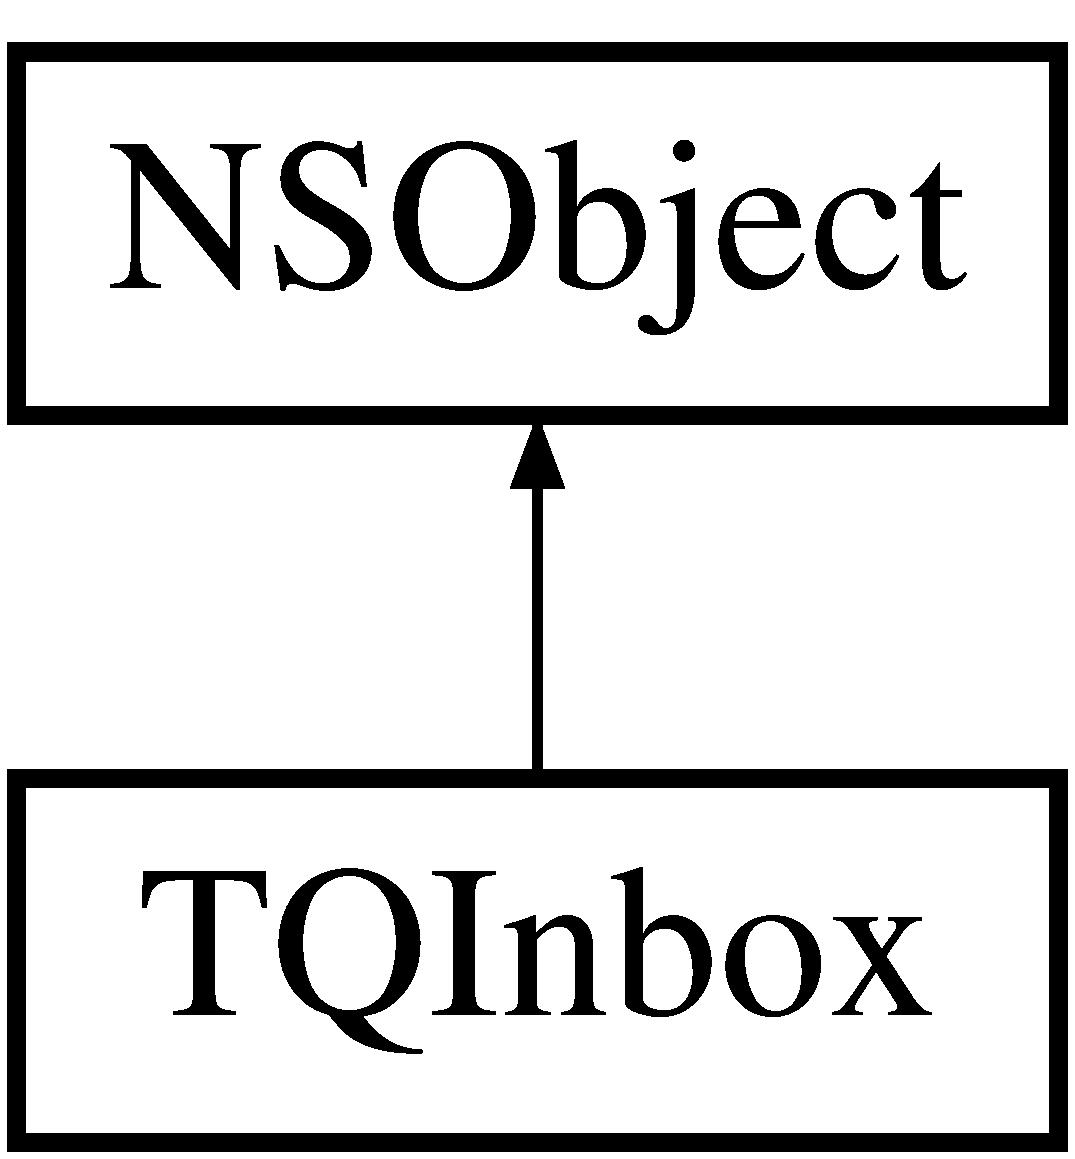
\includegraphics[height=2.000000cm]{interface_t_q_inbox}
\end{center}
\end{figure}
\subsection*{methods}
\begin{DoxyCompactItemize}
\item 
(\hyperlink{interface_t_q_inbox}{T\+Q\+Inbox} $\ast$) + \hyperlink{interface_t_q_inbox_addff5a4ce89ad34f6015c4f349ceb407}{shared}
\item 
(B\+O\+O\+L) -\/ \hyperlink{interface_t_q_inbox_a1e4abc18f0c11d2d47557448dae03113}{add\+Alert\+:fence\+Id\+:alert\+:action\+:}
\item 
(B\+O\+O\+L) -\/ \hyperlink{interface_t_q_inbox_a328211918a736eaf22cd1756f50adcb0}{add\+Alert\+:alert\+:}
\item 
(void) -\/ \hyperlink{interface_t_q_inbox_a0b13e889003893f499a099fe2605456f}{retrieve\+Custom\+Content\+:completion\+:}
\item 
(N\+S\+Array $\ast$) -\/ \hyperlink{interface_t_q_inbox_af74c125d553742be90efc16b3c0bf118}{get\+Inbox\+Messages\+:}
\item 
(\hyperlink{interface_t_q_inbox_message}{T\+Q\+Inbox\+Message} $\ast$) -\/ \hyperlink{interface_t_q_inbox_a06be946ff7d05d6a54eb0379e916d3fb}{get\+Inbox\+Message\+:}
\item 
(int) -\/ \hyperlink{interface_t_q_inbox_a949a8144d968545d7988cde6192ba33c}{get\+Inbox\+Messages\+Count\+:}
\item 
(B\+O\+O\+L) -\/ \hyperlink{interface_t_q_inbox_a64013736989134e4b7f778d2b2cc669d}{mark\+As\+Read\+:}
\item 
(B\+O\+O\+L) -\/ \hyperlink{interface_t_q_inbox_a7e716661eb1f0380af913bc5c65555d5}{mark\+As\+Unread\+:}
\item 
(int) -\/ \hyperlink{interface_t_q_inbox_a30780710283c7e6deceee5b786187e79}{remove\+Messages\+With\+Status\+:}
\item 
(B\+O\+O\+L) -\/ \hyperlink{interface_t_q_inbox_a3842fcc859c78bb50fd18ca0a39b290b}{remove\+Message\+:}
\item 
(B\+O\+O\+L) -\/ \hyperlink{interface_t_q_inbox_a01b262a134221af86ff3118b752486da}{add\+Custom\+Status\+:status\+:}
\end{DoxyCompactItemize}


\subsection{Detailed Description}
\hyperlink{interface_t_q_inbox}{T\+Q\+Inbox} Act as an inbox for pushes 

\subsection{Method Documentation}
\hypertarget{interface_t_q_inbox_a328211918a736eaf22cd1756f50adcb0}{}\index{T\+Q\+Inbox@{T\+Q\+Inbox}!add\+Alert\+:alert\+:@{add\+Alert\+:alert\+:}}
\index{add\+Alert\+:alert\+:@{add\+Alert\+:alert\+:}!T\+Q\+Inbox@{T\+Q\+Inbox}}
\subsubsection[{add\+Alert\+:alert\+:(\+N\+S\+String $\ast$push\+Id,[alert](deprecated) \+\_\+\+\_\+attribute\+\_\+\+\_\+)}]{\setlength{\rightskip}{0pt plus 5cm}-\/ (B\+O\+O\+L) add\+Alert\+: 
\begin{DoxyParamCaption}
\item[{(N\+S\+String $\ast$)}]{push\+Id}
\item[{alert:((deprecated))}]{\+\_\+\+\_\+attribute\+\_\+\+\_\+}
\end{DoxyParamCaption}
}\label{interface_t_q_inbox_a328211918a736eaf22cd1756f50adcb0}
add\+Alert Add an alert to the refenced push


\begin{DoxyParams}{Parameters}
{\em push\+Id} & the referenced push\textquotesingle{}s Id \\
\hline
{\em alert} & the alert to be added\\
\hline
\end{DoxyParams}
\begin{DoxyReturn}{Returns}
whether the transaction was successful or not 
\end{DoxyReturn}
\hypertarget{interface_t_q_inbox_a1e4abc18f0c11d2d47557448dae03113}{}\index{T\+Q\+Inbox@{T\+Q\+Inbox}!add\+Alert\+:fence\+Id\+:alert\+:action\+:@{add\+Alert\+:fence\+Id\+:alert\+:action\+:}}
\index{add\+Alert\+:fence\+Id\+:alert\+:action\+:@{add\+Alert\+:fence\+Id\+:alert\+:action\+:}!T\+Q\+Inbox@{T\+Q\+Inbox}}
\subsubsection[{add\+Alert\+:fence\+Id\+:alert\+:action\+:(\+N\+S\+String $\ast$push\+Id,[fence\+Id] N\+S\+String $\ast$fence\+Id,[alert] N\+S\+String $\ast$alert,[action] N\+S\+String $\ast$custom\+Action)}]{\setlength{\rightskip}{0pt plus 5cm}-\/ (B\+O\+O\+L) add\+Alert\+: 
\begin{DoxyParamCaption}
\item[{(N\+S\+String $\ast$)}]{push\+Id}
\item[{fenceId:(N\+S\+String $\ast$)}]{fence\+Id}
\item[{alert:(N\+S\+String $\ast$)}]{alert}
\item[{action:(N\+S\+String $\ast$)}]{custom\+Action}
\end{DoxyParamCaption}
}\label{interface_t_q_inbox_a1e4abc18f0c11d2d47557448dae03113}
add\+Alert Add an alert to the refenced push


\begin{DoxyParams}{Parameters}
{\em push\+Id} & the referenced push\textquotesingle{}s Id \\
\hline
{\em alert} & the alert to be added \\
\hline
{\em action} & the action if exists to be added\\
\hline
\end{DoxyParams}
\begin{DoxyReturn}{Returns}
whether the transaction was successful or not 
\end{DoxyReturn}
\hypertarget{interface_t_q_inbox_a01b262a134221af86ff3118b752486da}{}\index{T\+Q\+Inbox@{T\+Q\+Inbox}!add\+Custom\+Status\+:status\+:@{add\+Custom\+Status\+:status\+:}}
\index{add\+Custom\+Status\+:status\+:@{add\+Custom\+Status\+:status\+:}!T\+Q\+Inbox@{T\+Q\+Inbox}}
\subsubsection[{add\+Custom\+Status\+:status\+:(\+N\+S\+String $\ast$push\+Id,[status] N\+S\+String $\ast$status)}]{\setlength{\rightskip}{0pt plus 5cm}-\/ (B\+O\+O\+L) add\+Custom\+Status\+: 
\begin{DoxyParamCaption}
\item[{(N\+S\+String $\ast$)}]{push\+Id}
\item[{status:(N\+S\+String $\ast$)}]{status}
\end{DoxyParamCaption}
}\label{interface_t_q_inbox_a01b262a134221af86ff3118b752486da}
add\+Custom\+Status Add a custom status for the push in the database.


\begin{DoxyParams}{Parameters}
{\em push\+Id} & the referenced push\textquotesingle{}s id\\
\hline
{\em status} & the referenced push\textquotesingle{}s custom status\\
\hline
\end{DoxyParams}
\begin{DoxyReturn}{Returns}
if the push custom status was added or not 
\end{DoxyReturn}
\hypertarget{interface_t_q_inbox_a06be946ff7d05d6a54eb0379e916d3fb}{}\index{T\+Q\+Inbox@{T\+Q\+Inbox}!get\+Inbox\+Message\+:@{get\+Inbox\+Message\+:}}
\index{get\+Inbox\+Message\+:@{get\+Inbox\+Message\+:}!T\+Q\+Inbox@{T\+Q\+Inbox}}
\subsubsection[{get\+Inbox\+Message\+:(\+N\+S\+String $\ast$push\+Id)}]{\setlength{\rightskip}{0pt plus 5cm}-\/ ({\bf T\+Q\+Inbox\+Message} $\ast$) get\+Inbox\+Message\+: 
\begin{DoxyParamCaption}
\item[{(N\+S\+String $\ast$)}]{push\+Id}
\end{DoxyParamCaption}
}\label{interface_t_q_inbox_a06be946ff7d05d6a54eb0379e916d3fb}
get\+Inbox\+Message Gets an specific push through it\textquotesingle{}s identification


\begin{DoxyParams}{Parameters}
{\em push\+Id} & the referenced push\textquotesingle{}s Id\\
\hline
\end{DoxyParams}
\begin{DoxyReturn}{Returns}
a \hyperlink{interface_t_q_inbox_message}{T\+Q\+Inbox\+Message} with all the push\textquotesingle{}s information 
\end{DoxyReturn}
\hypertarget{interface_t_q_inbox_af74c125d553742be90efc16b3c0bf118}{}\index{T\+Q\+Inbox@{T\+Q\+Inbox}!get\+Inbox\+Messages\+:@{get\+Inbox\+Messages\+:}}
\index{get\+Inbox\+Messages\+:@{get\+Inbox\+Messages\+:}!T\+Q\+Inbox@{T\+Q\+Inbox}}
\subsubsection[{get\+Inbox\+Messages\+:(\+T\+Q\+Inbox\+Message\+Status status)}]{\setlength{\rightskip}{0pt plus 5cm}-\/ (N\+S\+Array $\ast$) get\+Inbox\+Messages\+: 
\begin{DoxyParamCaption}
\item[{(T\+Q\+Inbox\+Message\+Status)}]{status}
\end{DoxyParamCaption}
}\label{interface_t_q_inbox_af74c125d553742be90efc16b3c0bf118}
get\+Inbox\+Message Gets all the T\+Q\+Inbox\+Messages with a given status (see the enum defined)


\begin{DoxyParams}{Parameters}
{\em status} & the status the message should have to be retrieved\\
\hline
\end{DoxyParams}
\begin{DoxyReturn}{Returns}
an array containing all the matching T\+Q\+Inbox\+Messages not ordered 
\end{DoxyReturn}
\hypertarget{interface_t_q_inbox_a949a8144d968545d7988cde6192ba33c}{}\index{T\+Q\+Inbox@{T\+Q\+Inbox}!get\+Inbox\+Messages\+Count\+:@{get\+Inbox\+Messages\+Count\+:}}
\index{get\+Inbox\+Messages\+Count\+:@{get\+Inbox\+Messages\+Count\+:}!T\+Q\+Inbox@{T\+Q\+Inbox}}
\subsubsection[{get\+Inbox\+Messages\+Count\+:(\+T\+Q\+Inbox\+Message\+Status status)}]{\setlength{\rightskip}{0pt plus 5cm}-\/ (int) get\+Inbox\+Messages\+Count\+: 
\begin{DoxyParamCaption}
\item[{(T\+Q\+Inbox\+Message\+Status)}]{status}
\end{DoxyParamCaption}
}\label{interface_t_q_inbox_a949a8144d968545d7988cde6192ba33c}
get\+Inbox\+Message\+Count Gets the count of T\+Q\+Inbox\+Messages with a certain status. Faster than get\+Inbox\+Messages if only the count is necessary.


\begin{DoxyParams}{Parameters}
{\em status} & the status the \hyperlink{interface_t_q_inbox_message}{T\+Q\+Inbox\+Message} should have to be counted\\
\hline
\end{DoxyParams}
\begin{DoxyReturn}{Returns}
the count as an int
\end{DoxyReturn}
\begin{DoxyWarning}{Warning}
since the return is an int, it cannot receive messages 
\end{DoxyWarning}
\hypertarget{interface_t_q_inbox_a64013736989134e4b7f778d2b2cc669d}{}\index{T\+Q\+Inbox@{T\+Q\+Inbox}!mark\+As\+Read\+:@{mark\+As\+Read\+:}}
\index{mark\+As\+Read\+:@{mark\+As\+Read\+:}!T\+Q\+Inbox@{T\+Q\+Inbox}}
\subsubsection[{mark\+As\+Read\+:(\+N\+S\+String $\ast$push\+Id)}]{\setlength{\rightskip}{0pt plus 5cm}-\/ (B\+O\+O\+L) mark\+As\+Read\+: 
\begin{DoxyParamCaption}
\item[{(N\+S\+String $\ast$)}]{push\+Id}
\end{DoxyParamCaption}
}\label{interface_t_q_inbox_a64013736989134e4b7f778d2b2cc669d}
mark\+As\+Read Change a certain push\textquotesingle{}s status to \textquotesingle{}already read\textquotesingle{} (see defined enum).


\begin{DoxyParams}{Parameters}
{\em push\+Id} & the referenced push\textquotesingle{}s id\\
\hline
\end{DoxyParams}
\begin{DoxyReturn}{Returns}
if the push was updated to \textquotesingle{}already read\textquotesingle{} or not 
\end{DoxyReturn}
\hypertarget{interface_t_q_inbox_a7e716661eb1f0380af913bc5c65555d5}{}\index{T\+Q\+Inbox@{T\+Q\+Inbox}!mark\+As\+Unread\+:@{mark\+As\+Unread\+:}}
\index{mark\+As\+Unread\+:@{mark\+As\+Unread\+:}!T\+Q\+Inbox@{T\+Q\+Inbox}}
\subsubsection[{mark\+As\+Unread\+:(\+N\+S\+String $\ast$push\+Id)}]{\setlength{\rightskip}{0pt plus 5cm}-\/ (B\+O\+O\+L) mark\+As\+Unread\+: 
\begin{DoxyParamCaption}
\item[{(N\+S\+String $\ast$)}]{push\+Id}
\end{DoxyParamCaption}
}\label{interface_t_q_inbox_a7e716661eb1f0380af913bc5c65555d5}
mark\+As\+Unread Change a certain push\textquotesingle{}s status to \textquotesingle{}not read\textquotesingle{} (see defined enum).


\begin{DoxyParams}{Parameters}
{\em push\+Id} & the referenced push\textquotesingle{}s id\\
\hline
\end{DoxyParams}
\begin{DoxyReturn}{Returns}
if the push was updated to \textquotesingle{}not read\textquotesingle{} or not 
\end{DoxyReturn}
\hypertarget{interface_t_q_inbox_a3842fcc859c78bb50fd18ca0a39b290b}{}\index{T\+Q\+Inbox@{T\+Q\+Inbox}!remove\+Message\+:@{remove\+Message\+:}}
\index{remove\+Message\+:@{remove\+Message\+:}!T\+Q\+Inbox@{T\+Q\+Inbox}}
\subsubsection[{remove\+Message\+:(\+N\+S\+String $\ast$push\+Id)}]{\setlength{\rightskip}{0pt plus 5cm}-\/ (B\+O\+O\+L) remove\+Message\+: 
\begin{DoxyParamCaption}
\item[{(N\+S\+String $\ast$)}]{push\+Id}
\end{DoxyParamCaption}
}\label{interface_t_q_inbox_a3842fcc859c78bb50fd18ca0a39b290b}
remove\+Message Delete a certain push from the database.


\begin{DoxyParams}{Parameters}
{\em push\+Id} & the referenced push\textquotesingle{}s id\\
\hline
\end{DoxyParams}
\begin{DoxyReturn}{Returns}
if the push was deleted successfully or not 
\end{DoxyReturn}
\hypertarget{interface_t_q_inbox_a30780710283c7e6deceee5b786187e79}{}\index{T\+Q\+Inbox@{T\+Q\+Inbox}!remove\+Messages\+With\+Status\+:@{remove\+Messages\+With\+Status\+:}}
\index{remove\+Messages\+With\+Status\+:@{remove\+Messages\+With\+Status\+:}!T\+Q\+Inbox@{T\+Q\+Inbox}}
\subsubsection[{remove\+Messages\+With\+Status\+:(\+T\+Q\+Inbox\+Message\+Status status)}]{\setlength{\rightskip}{0pt plus 5cm}-\/ (int) remove\+Messages\+With\+Status\+: 
\begin{DoxyParamCaption}
\item[{(T\+Q\+Inbox\+Message\+Status)}]{status}
\end{DoxyParamCaption}
}\label{interface_t_q_inbox_a30780710283c7e6deceee5b786187e79}
remove\+Messages\+With\+Status Removes multiple messages from the database


\begin{DoxyParams}{Parameters}
{\em status} & R\+E\+A\+D, U\+N\+R\+E\+A\+D or A\+L\+L\\
\hline
\end{DoxyParams}
\begin{DoxyReturn}{Returns}
the number of rows affected by the deletion 
\end{DoxyReturn}
\hypertarget{interface_t_q_inbox_a0b13e889003893f499a099fe2605456f}{}\index{T\+Q\+Inbox@{T\+Q\+Inbox}!retrieve\+Custom\+Content\+:completion\+:@{retrieve\+Custom\+Content\+:completion\+:}}
\index{retrieve\+Custom\+Content\+:completion\+:@{retrieve\+Custom\+Content\+:completion\+:}!T\+Q\+Inbox@{T\+Q\+Inbox}}
\subsubsection[{retrieve\+Custom\+Content\+:completion\+:(\+N\+S\+String $\ast$push\+Id,[completion] void($^\wedge$completion)(\+B\+O\+O\+L success, T\+Q\+Inbox\+Message $\ast$message))}]{\setlength{\rightskip}{0pt plus 5cm}-\/ (void) retrieve\+Custom\+Content\+: 
\begin{DoxyParamCaption}
\item[{(N\+S\+String$\ast$)}]{push\+Id}
\item[{completion:(void($^\wedge$)(B\+O\+O\+L success, {\bf T\+Q\+Inbox\+Message} $\ast$message))}]{completion}
\end{DoxyParamCaption}
}\label{interface_t_q_inbox_a0b13e889003893f499a099fe2605456f}
retrieve\+Custom\+Content Retrieves a certain push\textquotesingle{}s content


\begin{DoxyParams}{Parameters}
{\em push\+Id} & the referenced push\textquotesingle{}s Id \\
\hline
{\em completion} & a block called after the content is retrieved that receives if the transaction was successful and the content itself \\
\hline
\end{DoxyParams}
\hypertarget{interface_t_q_inbox_addff5a4ce89ad34f6015c4f349ceb407}{}\index{T\+Q\+Inbox@{T\+Q\+Inbox}!shared@{shared}}
\index{shared@{shared}!T\+Q\+Inbox@{T\+Q\+Inbox}}
\subsubsection[{shared()}]{\setlength{\rightskip}{0pt plus 5cm}+ ({\bf T\+Q\+Inbox} $\ast$) shared 
\begin{DoxyParamCaption}
{}
\end{DoxyParamCaption}
}\label{interface_t_q_inbox_addff5a4ce89ad34f6015c4f349ceb407}
shared Return an instance of itself, initializating it if there is no \hyperlink{interface_t_q_inbox}{T\+Q\+Inbox} object. Since it\textquotesingle{}s an shared object, it\textquotesingle{}ll only create one.

\begin{DoxyReturn}{Returns}
a \hyperlink{interface_t_q_inbox}{T\+Q\+Inbox} object 
\end{DoxyReturn}


The documentation for this class was generated from the following files\+:\begin{DoxyCompactItemize}
\item 
T\+Q\+Inbox.\+h\item 
T\+Q\+Inbox.\+m\end{DoxyCompactItemize}

\hypertarget{interface_t_q_inbox_message}{}\section{T\+Q\+Inbox\+Message Class Reference}
\label{interface_t_q_inbox_message}\index{T\+Q\+Inbox\+Message@{T\+Q\+Inbox\+Message}}


{\ttfamily \#import $<$T\+Q\+Inbox.\+h$>$}

Inheritance diagram for T\+Q\+Inbox\+Message\+:\begin{figure}[H]
\begin{center}
\leavevmode
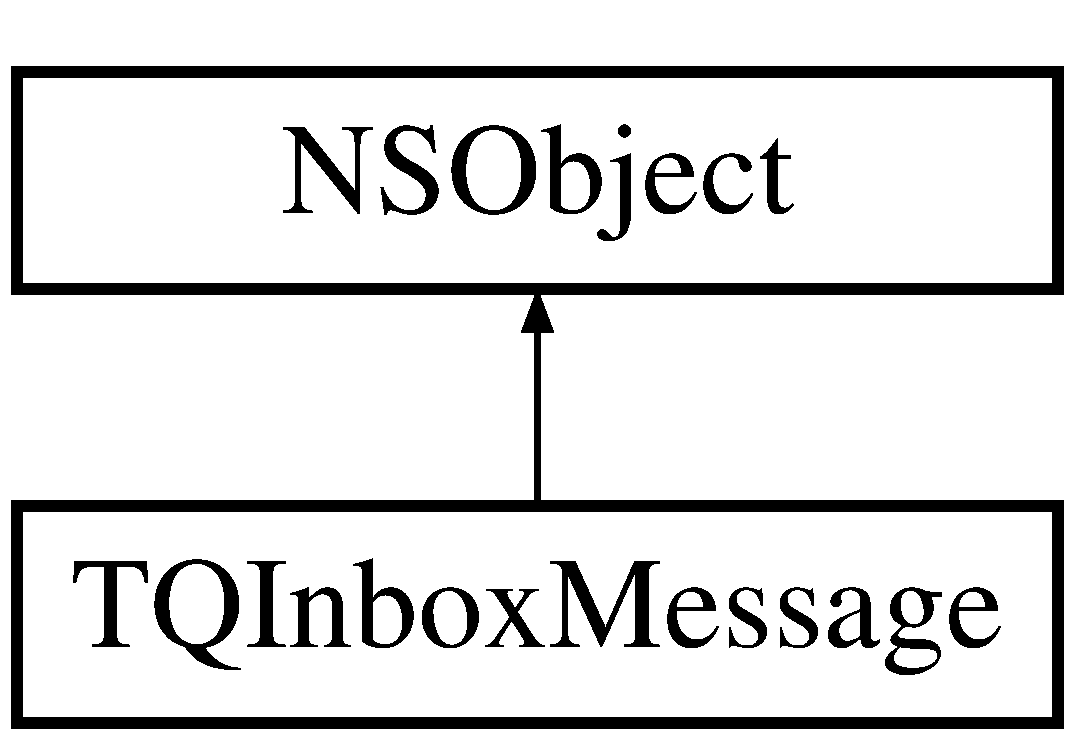
\includegraphics[height=2.000000cm]{interface_t_q_inbox_message}
\end{center}
\end{figure}
\subsection*{Instance Methods}
\begin{Indent}{\bf methods}\par
\begin{DoxyCompactItemize}
\item 
(\hyperlink{interface_t_q_inbox_message_a21a1990209c33c87dea6e82fb9878a29}{id}) -\/ \hyperlink{interface_t_q_inbox_message_aed6a33a1494e27e48a04191d9c12de37}{init\+With\+Push\+Id\+:fence\+Id\+:alert\+:content\+:type\+:status\+:complete\+:timestamp\+:scheduled\+:custom\+Status\+:custom\+Action\+:}
\end{DoxyCompactItemize}
\end{Indent}
\subsection*{Properties}
\begin{DoxyCompactItemize}
\item 
N\+S\+String $\ast$ \hyperlink{interface_t_q_inbox_message_a21a1990209c33c87dea6e82fb9878a29}{id}
\item 
N\+S\+String $\ast$ \hyperlink{interface_t_q_inbox_message_a167f2aee91be99c0ce08f980b80a0dba}{fence\+Id}
\item 
N\+S\+String $\ast$ \hyperlink{interface_t_q_inbox_message_a0fdd562c5d3ee1dba53743f893cadb36}{alert}
\item 
\hyperlink{interface_t_q_inbox_message_a21a1990209c33c87dea6e82fb9878a29}{id} \hyperlink{interface_t_q_inbox_message_a789f1e5b46d3121f8bbaaa69b05948fe}{content}
\item 
T\+Q\+Inbox\+Message\+Type \hyperlink{interface_t_q_inbox_message_a0095078f27cb8ac50a0306b83ef86ddc}{type}
\item 
T\+Q\+Inbox\+Message\+Status \hyperlink{interface_t_q_inbox_message_aef995a499d691cd27c255f59d68ec829}{status}
\item 
B\+O\+O\+L \hyperlink{interface_t_q_inbox_message_a1c0241c9106a9e9a19df35ad38d366ce}{complete}
\item 
int \hyperlink{interface_t_q_inbox_message_abd94ee3e5c563ce6a21fde6354c7337e}{timestamp}
\item 
int \hyperlink{interface_t_q_inbox_message_ad3ce8614fde9e7464af00f76bb59d685}{scheduled}
\item 
N\+S\+String $\ast$ \hyperlink{interface_t_q_inbox_message_a733ac6a53d04d9f8844438eae605cb76}{custom\+Sent\+Status}
\item 
N\+S\+String $\ast$ \hyperlink{interface_t_q_inbox_message_a473ac00dc8ef24707a418d3b480068b3}{custom\+Action}
\item 
(N\+S\+Array $\ast$) -\/ \hyperlink{interface_t_q_inbox_message_a53addd7d3427651e217fa76d8af3fee4}{get\+Custom\+Sent\+Status\+List}
\item 
(B\+O\+O\+L) -\/ \hyperlink{interface_t_q_inbox_message_a2f5a0d995823574eebbc87ab4f24fc83}{is\+Custom\+Status\+Sent\+:}
\end{DoxyCompactItemize}


\subsection{Detailed Description}
\hyperlink{interface_t_q_inbox_message}{T\+Q\+Inbox\+Message} Act as the push, storing it\textquotesingle{}s message, contents, and other data 

\subsection{Method Documentation}
\hypertarget{interface_t_q_inbox_message_a53addd7d3427651e217fa76d8af3fee4}{}\index{T\+Q\+Inbox\+Message@{T\+Q\+Inbox\+Message}!get\+Custom\+Sent\+Status\+List@{get\+Custom\+Sent\+Status\+List}}
\index{get\+Custom\+Sent\+Status\+List@{get\+Custom\+Sent\+Status\+List}!T\+Q\+Inbox\+Message@{T\+Q\+Inbox\+Message}}
\subsubsection[{get\+Custom\+Sent\+Status\+List()}]{\setlength{\rightskip}{0pt plus 5cm}-\/ (N\+S\+Array $\ast$) get\+Custom\+Sent\+Status\+List 
\begin{DoxyParamCaption}
{}
\end{DoxyParamCaption}
}\label{interface_t_q_inbox_message_a53addd7d3427651e217fa76d8af3fee4}
get\+Custom\+Sent\+Status\+List Get the custom status list that was already sent

\begin{DoxyReturn}{Returns}
Array with the sent custom status 
\end{DoxyReturn}
\hypertarget{interface_t_q_inbox_message_aed6a33a1494e27e48a04191d9c12de37}{}\index{T\+Q\+Inbox\+Message@{T\+Q\+Inbox\+Message}!init\+With\+Push\+Id\+:fence\+Id\+:alert\+:content\+:type\+:status\+:complete\+:timestamp\+:scheduled\+:custom\+Status\+:custom\+Action\+:@{init\+With\+Push\+Id\+:fence\+Id\+:alert\+:content\+:type\+:status\+:complete\+:timestamp\+:scheduled\+:custom\+Status\+:custom\+Action\+:}}
\index{init\+With\+Push\+Id\+:fence\+Id\+:alert\+:content\+:type\+:status\+:complete\+:timestamp\+:scheduled\+:custom\+Status\+:custom\+Action\+:@{init\+With\+Push\+Id\+:fence\+Id\+:alert\+:content\+:type\+:status\+:complete\+:timestamp\+:scheduled\+:custom\+Status\+:custom\+Action\+:}!T\+Q\+Inbox\+Message@{T\+Q\+Inbox\+Message}}
\subsubsection[{init\+With\+Push\+Id\+:fence\+Id\+:alert\+:content\+:type\+:status\+:complete\+:timestamp\+:scheduled\+:custom\+Status\+:custom\+Action\+:(\+N\+S\+String $\ast$id,[fence\+Id] N\+S\+String $\ast$fence\+Id,[alert] N\+S\+String $\ast$alert,[content] N\+S\+String $\ast$content,[type] T\+Q\+Inbox\+Message\+Type type,[status] T\+Q\+Inbox\+Message\+Status status,[complete] B\+O\+O\+L complete,[timestamp] int timestamp,[scheduled] int scheduled,[custom\+Status] N\+S\+String $\ast$custom\+Status,[custom\+Action] N\+S\+String $\ast$custom\+Action)}]{\setlength{\rightskip}{0pt plus 5cm}-\/ ({\bf id}) init\+With\+Push\+Id\+: 
\begin{DoxyParamCaption}
\item[{(N\+S\+String $\ast$)}]{id}
\item[{fenceId:(N\+S\+String $\ast$)}]{fence\+Id}
\item[{alert:(N\+S\+String $\ast$)}]{alert}
\item[{content:(N\+S\+String $\ast$)}]{content}
\item[{type:(T\+Q\+Inbox\+Message\+Type)}]{type}
\item[{status:(T\+Q\+Inbox\+Message\+Status)}]{status}
\item[{complete:(B\+O\+O\+L)}]{complete}
\item[{timestamp:(int)}]{timestamp}
\item[{scheduled:(int)}]{scheduled}
\item[{customStatus:(N\+S\+String $\ast$)}]{custom\+Status}
\item[{customAction:(N\+S\+String $\ast$)}]{custom\+Action}
\end{DoxyParamCaption}
}\label{interface_t_q_inbox_message_aed6a33a1494e27e48a04191d9c12de37}
init\+With\+Push\+Id instantiates an in-\/memory \hyperlink{interface_t_q_inbox_message}{T\+Q\+Inbox\+Message} representing the push


\begin{DoxyParams}{Parameters}
{\em id} & the referenced the push\textquotesingle{}s id \\
\hline
{\em alert} & the referenced push\textquotesingle{}s alert \\
\hline
{\em content} & the referenced push\textquotesingle{}s content \\
\hline
{\em type} & which type of content the push holds (see enum defined) \\
\hline
{\em status} & the referenced push\textquotesingle{}s status (see enum defined) \\
\hline
{\em complete} & the referenced push\textquotesingle{}s complete parameter \\
\hline
{\em timestamp} & the referenced push\textquotesingle{}s timestamp \\
\hline
{\em custom\+Sent\+Status} & the referenced push\textquotesingle{}s custom status \\
\hline
{\em custom\+Action} & the referenced push\textquotesingle{}s custom status\\
\hline
\end{DoxyParams}
\begin{DoxyReturn}{Returns}

\end{DoxyReturn}
\hypertarget{interface_t_q_inbox_message_a2f5a0d995823574eebbc87ab4f24fc83}{}\index{T\+Q\+Inbox\+Message@{T\+Q\+Inbox\+Message}!is\+Custom\+Status\+Sent\+:@{is\+Custom\+Status\+Sent\+:}}
\index{is\+Custom\+Status\+Sent\+:@{is\+Custom\+Status\+Sent\+:}!T\+Q\+Inbox\+Message@{T\+Q\+Inbox\+Message}}
\subsubsection[{is\+Custom\+Status\+Sent\+:(\+N\+S\+String $\ast$status)}]{\setlength{\rightskip}{0pt plus 5cm}-\/ (B\+O\+O\+L) is\+Custom\+Status\+Sent\+: 
\begin{DoxyParamCaption}
\item[{(N\+S\+String $\ast$)}]{status}
\end{DoxyParamCaption}
}\label{interface_t_q_inbox_message_a2f5a0d995823574eebbc87ab4f24fc83}
is\+Custom\+Status\+Sent Verify if a status was already sent


\begin{DoxyParams}{Parameters}
{\em status} & the referenced push\textquotesingle{}s custom status\\
\hline
\end{DoxyParams}
\begin{DoxyReturn}{Returns}
whether there status was already sent or not 
\end{DoxyReturn}


\subsection{Property Documentation}
\hypertarget{interface_t_q_inbox_message_a0fdd562c5d3ee1dba53743f893cadb36}{}\index{T\+Q\+Inbox\+Message@{T\+Q\+Inbox\+Message}!alert@{alert}}
\index{alert@{alert}!T\+Q\+Inbox\+Message@{T\+Q\+Inbox\+Message}}
\subsubsection[{alert}]{\setlength{\rightskip}{0pt plus 5cm}-\/ (N\+S\+String$\ast$) alert\hspace{0.3cm}{\ttfamily [read]}, {\ttfamily [atomic]}, {\ttfamily [assign]}}\label{interface_t_q_inbox_message_a0fdd562c5d3ee1dba53743f893cadb36}
Act as an inbox for pushes \hypertarget{interface_t_q_inbox_message_a1c0241c9106a9e9a19df35ad38d366ce}{}\index{T\+Q\+Inbox\+Message@{T\+Q\+Inbox\+Message}!complete@{complete}}
\index{complete@{complete}!T\+Q\+Inbox\+Message@{T\+Q\+Inbox\+Message}}
\subsubsection[{complete}]{\setlength{\rightskip}{0pt plus 5cm}-\/ (B\+O\+O\+L) complete\hspace{0.3cm}{\ttfamily [read]}, {\ttfamily [atomic]}, {\ttfamily [assign]}}\label{interface_t_q_inbox_message_a1c0241c9106a9e9a19df35ad38d366ce}
If the push\textquotesingle{}s data were all retrieved \hypertarget{interface_t_q_inbox_message_a789f1e5b46d3121f8bbaaa69b05948fe}{}\index{T\+Q\+Inbox\+Message@{T\+Q\+Inbox\+Message}!content@{content}}
\index{content@{content}!T\+Q\+Inbox\+Message@{T\+Q\+Inbox\+Message}}
\subsubsection[{content}]{\setlength{\rightskip}{0pt plus 5cm}-\/ ({\bf id}) content\hspace{0.3cm}{\ttfamily [read]}, {\ttfamily [atomic]}, {\ttfamily [assign]}}\label{interface_t_q_inbox_message_a789f1e5b46d3121f8bbaaa69b05948fe}
The push\textquotesingle{}s content. It can be an tag, link or simple message \hypertarget{interface_t_q_inbox_message_a473ac00dc8ef24707a418d3b480068b3}{}\index{T\+Q\+Inbox\+Message@{T\+Q\+Inbox\+Message}!custom\+Action@{custom\+Action}}
\index{custom\+Action@{custom\+Action}!T\+Q\+Inbox\+Message@{T\+Q\+Inbox\+Message}}
\subsubsection[{custom\+Action}]{\setlength{\rightskip}{0pt plus 5cm}-\/ (N\+S\+String$\ast$) custom\+Action\hspace{0.3cm}{\ttfamily [read]}, {\ttfamily [atomic]}, {\ttfamily [assign]}}\label{interface_t_q_inbox_message_a473ac00dc8ef24707a418d3b480068b3}
The custom\+Action id for the push notification \hypertarget{interface_t_q_inbox_message_a733ac6a53d04d9f8844438eae605cb76}{}\index{T\+Q\+Inbox\+Message@{T\+Q\+Inbox\+Message}!custom\+Sent\+Status@{custom\+Sent\+Status}}
\index{custom\+Sent\+Status@{custom\+Sent\+Status}!T\+Q\+Inbox\+Message@{T\+Q\+Inbox\+Message}}
\subsubsection[{custom\+Sent\+Status}]{\setlength{\rightskip}{0pt plus 5cm}-\/ (N\+S\+String$\ast$) custom\+Sent\+Status\hspace{0.3cm}{\ttfamily [read]}, {\ttfamily [atomic]}, {\ttfamily [assign]}}\label{interface_t_q_inbox_message_a733ac6a53d04d9f8844438eae605cb76}
The status already triggered with the push \hypertarget{interface_t_q_inbox_message_a167f2aee91be99c0ce08f980b80a0dba}{}\index{T\+Q\+Inbox\+Message@{T\+Q\+Inbox\+Message}!fence\+Id@{fence\+Id}}
\index{fence\+Id@{fence\+Id}!T\+Q\+Inbox\+Message@{T\+Q\+Inbox\+Message}}
\subsubsection[{fence\+Id}]{\setlength{\rightskip}{0pt plus 5cm}-\/ (N\+S\+String$\ast$) fence\+Id\hspace{0.3cm}{\ttfamily [read]}, {\ttfamily [atomic]}, {\ttfamily [assign]}}\label{interface_t_q_inbox_message_a167f2aee91be99c0ce08f980b80a0dba}
The fence id that generated the push (empty string if normal push) \hypertarget{interface_t_q_inbox_message_a21a1990209c33c87dea6e82fb9878a29}{}\index{T\+Q\+Inbox\+Message@{T\+Q\+Inbox\+Message}!id@{id}}
\index{id@{id}!T\+Q\+Inbox\+Message@{T\+Q\+Inbox\+Message}}
\subsubsection[{id}]{\setlength{\rightskip}{0pt plus 5cm}-\/ (N\+S\+String$\ast$) id\hspace{0.3cm}{\ttfamily [read]}, {\ttfamily [atomic]}, {\ttfamily [assign]}}\label{interface_t_q_inbox_message_a21a1990209c33c87dea6e82fb9878a29}
The push\textquotesingle{}s id in the database the \hyperlink{interface_t_q_inbox_message}{T\+Q\+Inbox\+Message} is related to \hypertarget{interface_t_q_inbox_message_ad3ce8614fde9e7464af00f76bb59d685}{}\index{T\+Q\+Inbox\+Message@{T\+Q\+Inbox\+Message}!scheduled@{scheduled}}
\index{scheduled@{scheduled}!T\+Q\+Inbox\+Message@{T\+Q\+Inbox\+Message}}
\subsubsection[{scheduled}]{\setlength{\rightskip}{0pt plus 5cm}-\/ (int) scheduled\hspace{0.3cm}{\ttfamily [read]}, {\ttfamily [atomic]}, {\ttfamily [assign]}}\label{interface_t_q_inbox_message_ad3ce8614fde9e7464af00f76bb59d685}
Moment that the notification was scheduled at \hypertarget{interface_t_q_inbox_message_aef995a499d691cd27c255f59d68ec829}{}\index{T\+Q\+Inbox\+Message@{T\+Q\+Inbox\+Message}!status@{status}}
\index{status@{status}!T\+Q\+Inbox\+Message@{T\+Q\+Inbox\+Message}}
\subsubsection[{status}]{\setlength{\rightskip}{0pt plus 5cm}-\/ (T\+Q\+Inbox\+Message\+Status) status\hspace{0.3cm}{\ttfamily [read]}, {\ttfamily [atomic]}, {\ttfamily [assign]}}\label{interface_t_q_inbox_message_aef995a499d691cd27c255f59d68ec829}
If the push was read or not. \hypertarget{interface_t_q_inbox_message_abd94ee3e5c563ce6a21fde6354c7337e}{}\index{T\+Q\+Inbox\+Message@{T\+Q\+Inbox\+Message}!timestamp@{timestamp}}
\index{timestamp@{timestamp}!T\+Q\+Inbox\+Message@{T\+Q\+Inbox\+Message}}
\subsubsection[{timestamp}]{\setlength{\rightskip}{0pt plus 5cm}-\/ (int) timestamp\hspace{0.3cm}{\ttfamily [read]}, {\ttfamily [atomic]}, {\ttfamily [assign]}}\label{interface_t_q_inbox_message_abd94ee3e5c563ce6a21fde6354c7337e}
When the push was modified \hypertarget{interface_t_q_inbox_message_a0095078f27cb8ac50a0306b83ef86ddc}{}\index{T\+Q\+Inbox\+Message@{T\+Q\+Inbox\+Message}!type@{type}}
\index{type@{type}!T\+Q\+Inbox\+Message@{T\+Q\+Inbox\+Message}}
\subsubsection[{type}]{\setlength{\rightskip}{0pt plus 5cm}-\/ (T\+Q\+Inbox\+Message\+Type) type\hspace{0.3cm}{\ttfamily [read]}, {\ttfamily [atomic]}, {\ttfamily [assign]}}\label{interface_t_q_inbox_message_a0095078f27cb8ac50a0306b83ef86ddc}
The push\textquotesingle{}s type. See the enum defined. 

The documentation for this class was generated from the following files\+:\begin{DoxyCompactItemize}
\item 
T\+Q\+Inbox.\+h\item 
T\+Q\+Inbox.\+m\end{DoxyCompactItemize}

%--- End generated contents ---

% Index
\backmatter
\newpage
\phantomsection
\clearemptydoublepage
\addcontentsline{toc}{chapter}{Index}
\printindex

\end{document}
